%%%%%%%%%%%%%%%%%%%%%%%%%%%%%%%%%%%%%%%%%
% Classicthesis Typographic Thesis
% LaTeX Template
% Version 1.1 (4/8/12)
%
% This template has been downloaded from:
% http://www.LaTeXTemplates.com
%
% Original author:
% André Miede (http://www.miede.de)
%
% License:
% CC BY-NC-SA 3.0 (http://creativecommons.org/licenses/by-nc-sa/3.0/)
%
% General Tips:
% 1) Make sure to edit the classicthesis-config.file
% 2) New enumeration (A., B., C., etc in small caps): \begin{aenumerate} \end{aenumerate}
% 3) For margin notes: \marginpar or \graffito{}
% 4) Do not use bold fonts in this style, it is designed around them
% 5) Use tables as in the examples
% 6) See classicthesis-preamble.sty for useful commands
%
%%%%%%%%%%%%%%%%%%%%%%%%%%%%%%%%%%%%%%%%%

%----------------------------------------------------------------------------------------
%	PACKAGES AND OTHER DOCUMENT CONFIGURATIONS
%----------------------------------------------------------------------------------------

\documentclass[
				twoside,openright,titlepage,numbers=noenddot,headinclude,%1headlines,
                footinclude=true,cleardoublepage=empty,
                BCOR=5mm,paper=a4,fontsize=9pt, % Binding correction, paper type and font size
                estonian,swedish,spanish,american, % Languages
                ]{scrreprt} 
                
% Includes the file which contains all the document configurations and packages - make sure to edit this file
%%%%%%%%%%%%%%%%%%%%%%%%%%%%%%%%%%%%%%%%%
% Configuration File
%
% The main lines to change in this file are in the DOCUMENT VARIABLES
% section, the rest of the file is for advanced configuration.
%
%%%%%%%%%%%%%%%%%%%%%%%%%%%%%%%%%%%%%%%%%

\PassOptionsToPackage{dottedtoc,eulerchapternumbers,pdfspacing,subfig,beramono,eulermath,parts}{classicthesis}

\newcommand{\myTitle}{Estonian Textbook\xspace}
\newcommand{\mySubtitle}{Traducci\'on no-oficial al espa\~nol \xspace}
\newcommand{\myName}{Juhan Tuldava \dag \xspace}
\newcommand{\myTime}{2013\xspace}
\newcommand{\myVersion}{versi\'on 0.00\xspace}

%----------------------------------------------------------------------------------------
%	USEFUL COMMANDS
%----------------------------------------------------------------------------------------

\newcommand{\ie}{i.\,e.}
\newcommand{\Ie}{I.\,e.}
\newcommand{\eg}{e.\,g.}
\newcommand{\Eg}{E.\,g.} 
\newcommand{\bemph}{\textbf}
\newcounter{dummy} % Necessary for correct hyperlinks (to index, bib, etc.)
\providecommand{\mLyX}{L\kern-.1667em\lower.25em\hbox{Y}\kern-.125emX\@}

%----------------------------------------------------------------------------------------
%	PACKAGES
%----------------------------------------------------------------------------------------

\usepackage{textcomp} % Used for special characters

%------------------------------------------------

\usepackage{lipsum} % Used for inserting dummy 'Lorem ipsum' text into the template

%------------------------------------------------
 
%\PassOptionsToPackage{latin9}{inputenc} % latin9 (ISO-8859-9) = latin1+"Euro sign"
\usepackage[utf8]{inputenc}
 
 %------------------------------------------------

%\PassOptionsToPackage{ngerman,american}{babel}  % Change this to your language(s)
% Spanish languages need extra options in order to work with this template
%\PassOptionsToPackage{spanish,es-lcroman}{babel}
\usepackage[swedish, estonian, spanish]{babel}
 
 %------------------------------------------------

\PassOptionsToPackage{T1}{fontenc} % T2A for cyrillics
\usepackage{fontenc}

%------------------------------------------------

\usepackage{xspace} % To get the spacing after macros right

%------------------------------------------------

\usepackage{mparhack} % To get marginpar right

%------------------------------------------------

\usepackage{fixltx2e} % Fixes some LaTeX stuff 

%------------------------------------------------

\PassOptionsToPackage{smaller}{acronym} % Include printonlyused in the first bracket to only show acronyms used in the text
\usepackage{acronym} % nice macros for handling all acronyms in the thesis

%------------------------------------------------

\PassOptionsToPackage{pdftex}{graphicx}
\usepackage{graphicx} 
  
%----------------------------------------------------------------------------------------
%	FLOATS: TABLES, FIGURES AND CAPTIONS SETUP
%----------------------------------------------------------------------------------------

\usepackage{tabularx} % Better tables
\setlength{\extrarowheight}{3pt} % Increase table row height
\newcommand{\tableheadline}[1]{\multicolumn{1}{c}{\spacedlowsmallcaps{#1}}}
\newcommand{\myfloatalign}{\centering} % To be used with each float for alignment
\usepackage{caption}
\captionsetup{format=hang,font=small}
\usepackage{subfig}

%----------------------------------------------------------------------------------------
%	HYPERREFERENCES
%----------------------------------------------------------------------------------------

\PassOptionsToPackage{pdftex,hyperfootnotes=false,pdfpagelabels}{hyperref}
\usepackage{hyperref}  % backref linktocpage pagebackref
\pdfcompresslevel=9
\pdfadjustspacing=1

\hypersetup{
% Uncomment the line below to remove all links (to references, figures, tables, etc)
%draft, 
colorlinks=true, linktocpage=true, pdfstartpage=3, pdfstartview=FitV,
% Uncomment the line below if you want to have black links (e.g. for printing black and white)
%colorlinks=false, linktocpage=false, pdfborder={0 0 0}, pdfstartpage=3, pdfstartview=FitV, 
breaklinks=true, pdfpagemode=UseNone, pageanchor=true, pdfpagemode=UseOutlines,
plainpages=false, bookmarksnumbered, bookmarksopen=true, bookmarksopenlevel=1,
hypertexnames=true, pdfhighlight=/O, urlcolor=webbrown, linkcolor=RoyalBlue, citecolor=webgreen,
%------------------------------------------------
% PDF file meta-information
pdftitle={\myTitle},
pdfauthor={\myName},
pdfsubject={},
pdfkeywords={},
pdfcreator={pdfLaTeX},
pdfproducer={LaTeX with hyperref and classicthesis}
%------------------------------------------------
}   

%----------------------------------------------------------------------------------------
%	BACKREFERENCES
%----------------------------------------------------------------------------------------

\usepackage{ifthen} % Allows the user of the \ifthenelse command
\newboolean{enable-backrefs} % Variable to enable backrefs in the bibliography
\setboolean{enable-backrefs}{false} % Variable value: true or false

\newcommand{\backrefnotcitedstring}{\relax} % (Not cited.)
\newcommand{\backrefcitedsinglestring}[1]{(Cited on page~#1.)}
\newcommand{\backrefcitedmultistring}[1]{(Cited on pages~#1.)}
\ifthenelse{\boolean{enable-backrefs}} % If backrefs were enabled
{
\PassOptionsToPackage{hyperpageref}{backref}
\usepackage{backref} % to be loaded after hyperref package 
\renewcommand{\backreftwosep}{ and~} % separate 2 pages
\renewcommand{\backreflastsep}{, and~} % separate last of longer list
\renewcommand*{\backref}[1]{}  % disable standard
\renewcommand*{\backrefalt}[4]{% detailed backref
\ifcase #1 
\backrefnotcitedstring
\or
\backrefcitedsinglestring{#2}
\else
\backrefcitedmultistring{#2}
\fi}
}{\relax} 

%----------------------------------------------------------------------------------------
%	AUTOREFERENCES SETUP
%	Redefines how references in text are prefaced for different 
%	languages (e.g. "Section 1.2" or "section 1.2")
%----------------------------------------------------------------------------------------

\makeatletter
\@ifpackageloaded{babel}
{
\addto\extrasamerican{
\renewcommand*{\figureautorefname}{Figure}
\renewcommand*{\tableautorefname}{Table}
\renewcommand*{\partautorefname}{Part}
\renewcommand*{\chapterautorefname}{Chapter}
\renewcommand*{\sectionautorefname}{Section}
\renewcommand*{\subsectionautorefname}{Section}
\renewcommand*{\subsubsectionautorefname}{Section}
}
\addto\extrasngerman{
\renewcommand*{\paragraphautorefname}{Absatz}
\renewcommand*{\subparagraphautorefname}{Unterabsatz}
\renewcommand*{\footnoteautorefname}{Fu\"snote}
\renewcommand*{\FancyVerbLineautorefname}{Zeile}
\renewcommand*{\theoremautorefname}{Theorem}
\renewcommand*{\appendixautorefname}{Anhang}
\renewcommand*{\equationautorefname}{Gleichung}
\renewcommand*{\itemautorefname}{Punkt}
}
\providecommand{\subfigureautorefname}{\figureautorefname} % Fix to getting autorefs for subfigures right
}{\relax}
\makeatother

%----------------------------------------------------------------------------------------

\usepackage{classicthesis} 

%----------------------------------------------------------------------------------------

\begin{document}

\frenchspacing % Reduces space after periods to make text more compact

\raggedbottom % Makes all pages the height of the text on that page

\selectlanguage{spanish} % Select your default language - e.g. american or ngerman

%\renewcommand*{\bibname}{new name} % Uncomment to change the name of the bibliography
%\setbibpreamble{} % Uncomment to include a preamble to the bibliography - some text before the reference list starts

\pagenumbering{roman} % Roman page numbering prior to the start of the thesis content (i, ii, iii, etc)

\pagestyle{plain} % Suppress headers for the pre-content pages

%----------------------------------------------------------------------------------------
%	PRE-CONTENT THESIS PAGES
%----------------------------------------------------------------------------------------

% Title Page

\begin{titlepage}

\begin{addmargin}[-1cm]{-3cm}
\begin{center}
\large

\hfill
\vfill

\begingroup
\color{MidnightBlue}\spacedallcaps{\myTitle} \\ \bigskip % Book title
\endgroup

\spacedlowsmallcaps{\myName} % Author's name

\vfill

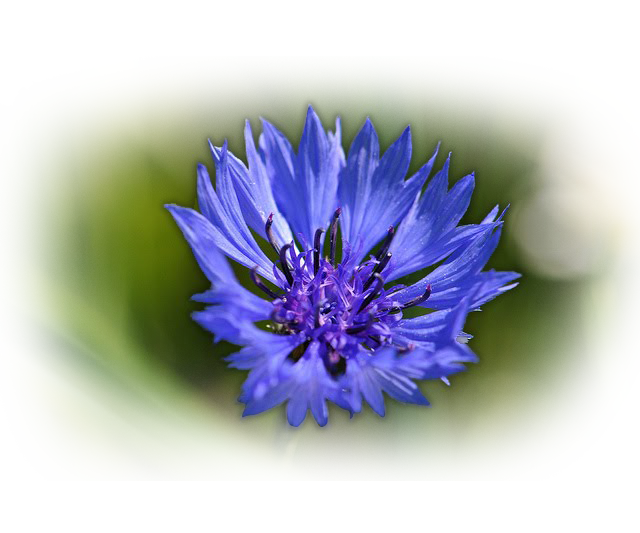
\includegraphics[width=10cm]{img/Estonian_Flower.png} \\ \medskip % Picture

\mySubtitle \\ \medskip % Book subtitle

\myTime\ -- \myVersion % Time and version

\vfill

\end{center}
\end{addmargin}

\end{titlepage}
 % Main title page

% Back of the title page

\thispagestyle{empty}

\hfill

\vfill

\noindent\myName: \textit{\myTitle,} \mySubtitle, %\myDegree, 
\textcopyright\ \myTime % Back of the title page

\cleardoublepage% Dedication

\thispagestyle{empty}
\refstepcounter{dummy}

\pdfbookmark[1]{Dedicatoria}{Dedicatoria} % Bookmark

\vspace*{3cm}

\begin{center}
Ükskord me võidame, niikuinii! \\ \medskip
--- Heinz Valk
\end{center}

\medskip

\begin{center}
Este libro está dedicado a todas aquellas personas que deseen sumergirse en este fascinante y hermoso idioma.
\end{center}
 % Dedication page

\cleardoublepage% Acknowledgements

\pdfbookmark[1]{Agradecimientos}{Agradecimientos} % Bookmark 

\chapter*{Agradecimientos} 

\lipsum[7]

Probanfo las citas \cite{bentley:1999}. \\
Probanfo las citas \cite{bringhurst:2002} . \\
Probanfo las citas \cite{cormen:2001} . \\
Probanfo las citas \cite{dueck:trio} . \\
Probanfo las citas \cite{knuth:1976} . \\
Probanfo las citas \cite{knuth:1974} . \\
Probanfo las citas \cite{sommerville:1992} . \\

%\noindent Más agradecimientos aquí \\
 % Acknowledgements page

%\cleardoublepage\include{FrontBackMatter/Abstract} % Abstract page

\cleardoublepage\include{FrontBackMatter/Publication} % Publications from the thesis page

\cleardoublepage% License

\thispagestyle{empty}
\refstepcounter{dummy}

\pdfbookmark[1]{Licencia}{Licencia} % Bookmark

\vspace*{3cm}

\begin{center}
 
\includegraphics[width=3cm]{img/by-nc-sa.pdf}\\ \bigskip
 El presente libro se distribuye con licencia \href{http://creativecommons.org/licenses/by-nc-sa/3.0/}{Creative Commons BY-NC-SA}
\end{center}

\pagestyle{scrheadings} % Show chapter titles as headings

\cleardoublepage% Table of Contents - List of Tables/Figures/Listings and Acronyms

\refstepcounter{dummy}

\pdfbookmark[1]{\contentsname}{tableofcontents} % Bookmark name visible in a PDF viewer

\setcounter{tocdepth}{2} % Depth of sections to include in the table of contents - currently up to subsections

\setcounter{secnumdepth}{3} % Depth of sections to number in the text itself - currently up to subsubsections

\manualmark
\markboth{\spacedlowsmallcaps{\contentsname}}{\spacedlowsmallcaps{\contentsname}}
\tableofcontents 
\automark[section]{chapter}
\renewcommand{\chaptermark}[1]{\markboth{\spacedlowsmallcaps{#1}}{\spacedlowsmallcaps{#1}}}
\renewcommand{\sectionmark}[1]{\markright{\thesection\enspace\spacedlowsmallcaps{#1}}}

\clearpage

\begingroup 
\let\clearpage\relax
\let\cleardoublepage\relax
\let\cleardoublepage\relax
                   
\endgroup

\cleardoublepage
 % Contents, list of figures/tables/listings and acronyms

\pagenumbering{arabic} % Arabic page numbering for thesis content (1, 2, 3, etc)

\cleardoublepage% Foreword

\pdfbookmark[1]{Foreword}{Foreword} % Bookmark name visible in a PDF viewer

\chapter*{Prólogo} % Foreword name

Durante siglos, los estonios han tenido contacto cercano con otras nacionalidades que viven en la zona del Mar Báltico al noreste de Europa. Entre las dos Guerras Mundiales (cuando Estonia era independiente), se fortalecieron los contactos políticos, económicos y culturales con los países vecinos. Incluso los contactos personales se desarrollaron, en gran medida, debido al turismo. Los mismos procesos se haces aún más evidentes hoy en día, después de que Estonia recuperara su independencia de la Unión Soviética en 1991.\\

A finales de la Segunda Guerra Mundial, decenas de miles de estonios huyeron a Suecia y Alemania. Muchos de ellos se instalaron en los Estados Unidos de América, Canadá y Australia. Fueron recibidos con amistad y entendimiento en los países donde buscaron refugio. En sus actividades laborales y de ocio diarios, los estonios se adaptaron bien a la vida en otros países, y la mayoría de ellos son ahora ciudadanos de sus nuevas patrias.\\

Los estonios en el extranjero no han olvidado su origen o su lengua. Quieren preservar su patrimonio cultural y mantener sus tradiciones. La colección de folclore de Estonia, por ejemplo, es uno de los más grandes del mundo, y los estonios en el extranjero con orgullo cuentan a sus hijos y amigos sobre el legendario héroe cuyas hazañas se registran en el épico folclore Kalevipoeg. Hay incluso una extensa y muy rica variedad de literatura estonia moderna, aunque poco de ella ha sido traducida a otros idiomas aún. Músicos y cantantes de Estonia son excepcionales, y grandes festivales en su patria así como en el extranjero reúnen a miles de miembros del coro, bailarines folclóricos, y gimnastas rítmicos para ganar fama por sus actuaciones. Anticuadas artesanías estonias también han llamado la atención - particularmente las artes textiles, cuero, madera y orfebrería. Muchos artistas y estudiosos contemporáneos han ganado reconocimiento internacional, por trabajos relacionados o inspirados por las viejas tradiciones y nuevos desarrollos en Estonia.\\

La lengua estonia pertenece a la familia ugrofinesa, junto con el finés, el húngaro, las lenguas sami (lapón), y un número de otras lenguas habladas por los pueblos dispersos en el norte de Rusia. Las lenguas de los pueblos cercanos - ruso, letón, lituano, sueco - se encuentran en un grupo diferente, llamada la familia indoeuropea. El inglés también se encuentra en esta última familia, lo que significa que su estructura difiere en importantes aspectos de la lengua estonia. Sin embargo, no es tan difícil para una persona de habla inglesa aprender estonio como generalmente se cree.\\

Este libro está destinado principalmente para los estadounidenses y otros hablantes del inglés que, por diversas razones, están interesados en el idioma estonio. En la preparación de este libro, sin embargo, el autor también tuvo en cuenta la generación más joven de los estonios residentes en el extranjero, sin la oportunidad de aprender la gramática del estonio en las escuelas a las que asisten.\\

El libro se puede utilizar para el estudio independiente, pero para un aprendizaje óptimo, se recomienda la ayuda de una persona de habla estonia, sobre todo al principio. En caso de que el libro se utilice en un curso, el instructor puede cambiar el orden de los temas o añadir más ejercicios según sea necesario.\\

El libro contiene 40 lecciones, cada una de las cuales tiene seis secciones: gramática, texto (selección de lectura), vocabulario, ejercicios (diseñado para reforzar el aprendizaje tanto de gramática como de vocabulario), expresiones (elegidas acorde a la gramática del capítulo en mente, y a menudo agrupados por tema), y las respuestas a los ejercicios.\\

En las secciones de gramática, el autor ha tratado de presentar las principales características de la gramática estonia de la forma más sencilla posible. Para hacer las cosas más claras, las comparaciones con las reglas de la gramática inglesa se hacen a menudo.\\

Aquellos que no tienen deseo ni tiempo para un estudio profundo de la gramática estonia pero que desean ampliar su repertorio de frases coloquiales y palabras comunes encontrará el tema de las expresiones de cada lección (Saludos y Agradecimientos, Comidas y Bebidas, Tiempo, Clima, Correspondencias, Enfermedad , Oficio, etc.) listadas en la tabla de contenidos. El índice también enumera los temas tratados en las lecturas y las listas de expresiones.\\

Las selecciones de lectura, mayormente composiciones originales hechas por el autor, están diseñadas para reforzar los puntos de la gramática. Las cursivas se utilizan para identificar las palabras o frases que ilustran las formas gramaticales presentadas en la misma lección. Al mismo tiempo, el autor ha tratado de cubrir un amplio rango de temas y situaciones para construir el vocabulario del alumno tanto como sea posible para una conversación regular.\\

Al final del libro se incluye un diccionario general de Estonia-Inglés, con todos los términos presentados en la lista de vocabulario de cada capítulo y otras palabras comunes. Para la traducción de palabras del inglés al estonio, el estudiante necesitará un diccionario Inglés-Estonio. Una breve revisión de los términos gramaticales también se presenta al final. El índice consta de dos partes, con listados alfabéticos separados en términos gramaticales y temas de conversación.\\

La idea de escribir un libro sobre el estonio se presentó en el verano de 1960 en el curso de la Escuela de Continuación Estonia (Estniska Folkhögskolan) en Gimo, Suecia, donde el autor enseñó estonio por varios años y por lo mismo obtuvo la perspicacia sobre las dificultades de instruir a los jóvenes sin previo estudio de la gramática estonia.\\

La fuente de inspiración fue ombudsman Nils Hellstrom, y estoy muy agradecido con él, no sólo por surgir con la idea de este libro, sino también por organizar su primera publicación (en 1962) a través de Bokförlaget Medborgarskolan. También deseo expresar mis agradecimientos al director Henry Jarild, por su cooperación y ayuda en relación con la publicación original de este libro.\\

Quiero expresar un especial agradecimiento a Gita Aasmaa y Tarmo Oja, no sólo por proporcionar diversas formas de asistencia técnica, sino también por contribuir puntos de vista muy valiosos y sugerencias con respecto al contenido del libro.\\

Estoy especialmente agradecido con el profesor Ain Haas por asumir y llevar a cabo extremadamente bien la enorme tarea de traducir y actualizar el libro de esta edición.\\

\hfill \textit{Juhan Tuldava}

\hfill Tartu, Estonia			

\vfill
 % Uncomment and create a Foreword.tex to include a foreword

\cleardoublepage% Translation Notes

\pdfbookmark[1]{Translation}{Translation} % Bookmark name visible in a PDF viewer

\chapter*{Nota del Traductor} % Translation Notes name

Varios libros están disponibles para las personas que desean estudiar el idioma Estonio. Cualquier persona seria en el asunto no debería pasar por alto el trabajo del profesor Tuldava. En el esfuerzo por mejorar mi dominio del estonio, no encontré nada más valioso que su libro. Es verdaderamente impresionante en su claridad, rigurosidad y lógica de progresión. Provee un riguroso curso de instrucciones, equivalente a dos años universitarios, pero tiene muchos giros interesantes e incluso toques humorísticos que hacen las lecciones agradables.\\

Después de descubrir el libro durante un viaje de investigación a Suecia, llegué a sentir que merecía una distribución mucho más amplia. Como un Estonio nacido en Suecia y criado en los Estados Unidos, con fluidez en los tres idiomas, me encontré en una buena posición para preparar una versión en Inglés de este excelente libro, para el beneficio de los familiares y amigos en los EE.UU. que no pudieron hacer uso de la versión sueca. Debido a su apoyo, así como un creciente número de solicitudes de otras partes, he decidido hacer mi traducción a disposición de un público más amplio. El creciente interés por la lengua entre todo tipo de personas que no tienen una conexión ancestral con el país refleja la nueva situación de Estonia como país europeo vanguardista haciendo grandes avances para superar el legado de la ocupación soviética.\\

La versión en Inglés es básicamente la misma que la versión sueca, pero se hicieron algunos cambios en la preparación de esta traducción. Sustituí referencias a nombres de Estados Unidos, ubicaciones, divisas, etc. de muchas de las originales suecas, y me tomé la libertad de añadir algunas expresiones que había encontrado en mi análisis de diccionarios y literatura de Estonia. Se han quitado puntos de la gramática aplicable solo a la lengua sueca, y han sido agregados nuevos comentarios sobre la gramática del Inglés. Para que sea más fácil utilizar el libro para el estudio independiente, he desarrollado un conjunto más completo de respuestas a los ejercicios y ampliado el glosario.\\

Durante una temporada como profesor visitante de sociología en la Universidad de Tartu en la primavera de 1993, me aproveché de la oportunidad para reunirme con el profesor Tuldava, quien recientemente se retiró como jefe del Departamento de Lenguas Germánicas. Hablamos sobre cómo actualizar y mejorar la publicación original sueca. Sus sugerencias - incluyendo algunos nuevos puntos sobre gramática que reflejan el uso cambiante en Estonia - se han incorporado en la versión.\\

Me gustaría expresar un especial agradecimiento al profesor Tuldava y a mi madre, Elly (Ratas) Haas, por comprobar cuidadosamente el manuscrito en varias etapas y ofrecer muchas sugerencias útiles.\\

Es con gran placer y orgullo que ofrezco esta traducción del libro del profesor Tuldava, a todos aquellos que busquen una llave para abrir los misterios del idioma Estonio y abrir la puerta a un mundo oculto de fascinante folclore, buena literatura y agradables conversaciones. Hay más de un millón de hablantes del idioma Estonio en el mundo hoy en día, y es mi mayor anelo que algunos más se animen a unirse a sus filas como resultado de este libro.\\

\hfill \textit{Ain Haas}

\hfill Indianapolis, USA.			

\vfill
 

\cleardoublepage% Abreviations & Symbols

\pdfbookmark[1]{Abreviaturas y Símbolos}{Abreviaturas y Simbolos} % Bookmark name visible in a PDF viewer

\chapter*{Abreviaturas y Símbolos} % Abreviations & Symbols name

\begin{tabular}{ l l }
	\begin{tabular}{ l c l }
	abbr.	& = & abreviatura \\
	abess.	& = & abesivo \\
	abl.	& = & ablativo \\
	adess.	& = & adesivo \\
	adj.	& = & adjetivo \\
	adv.	& = & adverbio \\
	all.	& = & alativo \\
	comit.	& = & comitativo \\
	comp.	& = & comparativo \\
	conj.	& = & conjunción \\
	cont.	& = & continuado \\
	dim.	& = & diminutivo \\
	e.g.	& = & por ejemplo \\
	elat.	& = & elativo \\
	emph.	& = & enfático \\
	etc.	& = & etcétera \\
	gen.	& = & genitivo \\
	i.e.	& = & en esencia \\
	ill.	& = & ilativo \\
	imper.	& = & imperativo \\
	imperf.	& = & imperfecto \\
	indecl.	& = & indeclinable \\
	iness.	& = & inesivo \\
	inf.	& = & infinitivo \\
	interj.	& = & interjección
	\end{tabular}
&
	\begin{tabular}{ l c l }
	lit.	& = & literalmente \\
	n.		& = & sustantivo \\
	neg.	& = & negativo \\
	nom.	& = & nominativo \\
	num.	& = & número \\
	part.	& = & partitivo \\
	partic.	& = & participio \\
	pass.	& = & pasivo \\
	perf.	& = & perfecto \\
	pers.	& = & persona \\
	pl.		& = & plural \\
	postp.	& = & posposición \\
	prep.	& = & preposición \\
	pres.	& = & presente \\
	pron.	& = & pronombre \\
	refl.	& = & reflexivo \\
	sing.	& = & singular \\
	superl.	& = & superlativo \\
	term.	& = & terminativo \\
	transl.	& = & translativo \\
	v.		& = & verbo \\
	v.i.	& = & verbo intransitivo \\
	vs.		& = & versus \\
	v.t.	& = & verbo transitivo
	\end{tabular}
\end{tabular}\\ \bigskip

\begin{tabular}{ l p{10cm} }
	\textasciiacute & indica que la tensión está en una sílaba dada, en contraste con el patrón habitual de hacer hincapié en la primera sílaba. \\
	\textasciigrave & indica un sonido extra largo (tercer grado) en la sílaba que sigue. \\
	\textquotesingle & indica palatalización de consonante. \\
	\S & significa sección.
\end{tabular}		

\vfill
 

\pagenumbering{arabic} % Arabic page numbering for thesis content (1, 2, 3, etc)
%\setcounter{page}{90} % Uncomment to manually start the page counter at an arbitrary value (for example if you wish to count the pre-content pages in the page count)

\cleardoublepage % Avoids problems with pdfbookmark

%----------------------------------------------------------------------------------------
%	BOOK CONTENT - LESSONS
%----------------------------------------------------------------------------------------

\ctparttext{Dentro de esta primera parte se expondrán la introducción y las 40 lecciones principales que constituyen el fuerte del libro. Es altamente recomendable realizar los ejercicios propuestos al final de cada lección, pues ayuda a decantar la teoría expuesta en la misma y proporciona un escenario real de aplicación.} 

\part{Manual Estonio} 

% ======================================
%
% 				Introduction
%
% ======================================

\pdfbookmark[1]{Introducción}{Introducción} % Bookmark name visible in a PDF viewer

\chapter*{Introducción} 

%----------------------------------------------------------------------------------------

\begin{enumerate}
	\item El alfabeto estonio básico consta de 23 letras en el siguiente orden:
	\begin{center}
	\begin{otherlanguage}{estonian}
		\bemph{a b c d e g h i j k l m n o p r s t u v õ ä ö ü}
	\end{otherlanguage}
	\end{center}

	Existen otras 9 letras que aparecen en las palabras extranjeras. Las letras \bemph{c q w x y} se encuentran sólo en los nombres extranjeros, como César, Don Quijote, Xantippe, Nueva York. Las letras \bemph{f š z ž} se encuentran en las palabras adoptadas de otros idiomas: film, šokolaad, zooloog, žurnaal.\\ 
	Finalmente, el orden del alfabeto completo es el siguiente:
	\begin{center}
	\begin{otherlanguage}{estonian}
		\bemph{a b c d e f g h i j k l m n o p q r s š z ž t u v w õ ä ö ü x y}
	\end{otherlanguage}
	\end{center}

	\item La mayoría de las letras se pronuncian de manera bastante similar al español. Sin embargo, tenga en cuenta lo siguiente:

	\section*{\Large{Vocales}}

	Las vocales \bemph{a e i o u} se pronuncian exactamente igual que en español, sin embargo la fonética de las vocales \bemph{ä õ ö ü} puede presentar una gran dificultad.\\

	La vocal \bemph{ä} se genera al intentar pronunciar las vocales \bemph{a} y \bemph{e} al mismo tiempo: \bemph{\ae}.\\

	La vocal \bemph{ö} se genera pronunciando la vocal \bemph{e} pero redondeando los labios como si se fuera a pronunciar la vocal \bemph{o}.\\

	La vocal \bemph{ü} se genera pronunciando la vocal \bemph{i} pero redondeando los labios como si se fuera a pronunciar la vocal \bemph{u}.\\

	La vocal \bemph{õ} se genera pronunciando la vocal \bemph{o} pero sin redondear los labios, como si se fuera a pronunciar la vocal \bemph{e}.\\

	Por supuesto lo más recomendable, más que leer una descripción, es escuchar el audio de las pronunciaciones de las vocales. El siguiente \href{http://www.youtube.com/watch?v=GfxrR45yA6I}{video}\footnote{http://www.youtube.com/watch?v=GfxrR45yA6I}, cortesía de \href{http://www.engetranslations.ee/airien.htm}{Airi Enge}\footnote{http://www.engetranslations.ee/airien.htm}, presenta de forma clara y precisa todas las vocales del estonio.\\

 	\section*{\Large{Consonantes}}

 	La constante \bemph{z} se pronuncia igual que la palabra inglesa `zoo'.\\

 	La constante \bemph{j} se pronuncia como la letra \bemph{y} en la palabra `maya'.\\

 	La constante \bemph{h} posee diferentes casos. Si está al principio de una palabra el sonido es muy débil, casi un silencio. Si está en medio de dos vocales se pronuncia como la \bemph{j} en la interjección coloquial `¡Ajá!', y si se encuentra antes de una consonante o al final de una palabra su pronunciación se torna más como una exhalación muy suave, haciendo amagos en formar una \bemph{j}.\\

 	Las consonantes \bemph{b d g} son sordas y ligeramente más suaves que las letras del español \bemph{p t k}, respectivamente.\\

 	Las consonantes \bemph{p t k} también son sordas, pero ligeramente más fuertes que las del español. Un sonido más duradero y ligeramente más potente se da en el caso de tener consonantes dobles \bemph{pp tt kk}\\

 	La consonante \bemph{š} equivale a la combinación \bemph{sh} en inglés, como en la palabra `english'.\\

 	La consonante \bemph{ž} equivale a la letra \bemph{s} en la palabra inglesa `treasure', o como la \bemph{j} de la palabra francesa `jour'.\\

 	Las consonantes \bemph{l r s m n v} se pronuncian exactamente igual que en español.\\

 	Las consonantes \bemph{f c q w x y} dependen del idioma del cual provienen.\\

 	\item En el estonio hay muchos diptongos o combinaciones de dos vocales que forman parte de la misma sílaba. Estos incluyen \bemph{ae ai ao au ea ei eo iu oa oe oi õe äe} y así sucesivamente. Cada una de las dos vocales se pronuncia con claridad, pero no como si estuvieran en sílabas distintas.\\

 	Ejemplos: laud, laev, hea, loen, õun, õed, käed.\\

 	\item La acentuación en el estonio, a diferencia del español, se encuentra normalmente en la primera sílaba. Hay, sin embargo, algunas excepciones como \foreignlanguage{estonian}{ai\bemph{täh} `gracias', sõb\bemph{ran}na `amiga', üle\bemph{üld}se `sobre todo'}. El acento de muchas palabras adoptadas de otros idiomas se ha mantenido: e\bemph{lek}ter, ide\bemph{aal}, pro\bemph{fes}sor. Cuando la marca \textasciiacute\ es usada en el texto sobre una vocal (como en elékter, ideáal, proféssor), indica que el acento está sobre esa sílaba, sin embargo esta marca no es parte de la ortografía normal.\\

 	\item La ortografía del estonio es fundamentalmente fonética, lo que significa que las palabras están escritas como suenan. Como una regla básica, letras solas significan sonidos cortos y letras dobles indican sonidos largos.\\

 	La pronunciación de las vocales individuales siempre es muy corto (primer grado), en contraste con las interminables vocales de palabras en inglés como `go', `at', `find'.\\

 	\item Vocales dobles, consonantes dobles y diptongos son largos (segundo grado) o muy largos (tercer grado).\\

 	Cada vocal y consonante en el estonio puede tener por lo tanto tres diferentes largos o grados:\\

 	\begin{tabular}{ r l l c l l}
 		1\textordmasculine\ grado: & s\bemph{a}da 					& `cien' 		& & li\bemph{n}a 					& `mantel, sábana' \\
 		2\textordmasculine\ grado: & s\bemph{aa}da 					& `¡envía!' 	& & li\bemph{nn}a 					& `ciudades' \\
 		3\textordmasculine\ grado: & \textasciigrave s\bemph{aa}da 	& `obtener' 	& & \textasciigrave li\bemph{nn}a 	& `hacia la ciudad' 
 	\end{tabular}

 	El tercer grado es notablemente más largo que los sonidos correspondientes al español o el inglés.\\

	En la transcripción fonética, el tercero grado se indican con una \textasciigrave\ antes de la sílaba. Esto no se utiliza en el lenguaje escrito, pero se utiliza en los diccionarios y listas de palabras en los casos en que la longitud afecta el significado. Por ejemplo: \textasciigrave Kooli (pronunciado como si hubieran 3 vocales - koooli) significa `a la escuela', en comparación con Kooli (pronunciado con sólo dos vocales) que significa `de la escuela'.\\

	\item En algunas palabras, las consonantes \bemph{l n s t} se suavizan o palatalizan con un ligero \bemph{i} o \bemph{j} (la \bemph{j} estonia) antes de la consonante.\\

	\begin{tabular}{ l l}
	Ejemplos: 	& palk (pal\textquotesingle k) `tronco, viga' \\
				& tund (tun\textquotesingle d) `hora' \\
				& kott (kot\textquotesingle t) `bolsa' \\
				& kass (kas\textquotesingle s) `gato' 
	\end{tabular}

	Este ablandamiento o palatalización no está indicado en el lenguaje escrito, pero se observa en los diccionarios y listas de palabras como una apóstrofe después de la consonante palatalizada, en los casos en que el significado de la palabra puede ser afectada: pal\textquotesingle k (con suavizado \bemph{i}) `tronco, viga', en comparación con palk (con una \bemph{i} normal no ablandada) `salario'.

\end{enumerate}	

\vfill
% ======================================
%
% 				Lesson 1
%
% ======================================

\chapter{Primera Lección}

\label{ch:lesson01} % For referencing the chapter elsewhere, use \autoref{ch:lesson01} 

%----------------------------------------------------------------------------------------

% =====================
% 		GRAMATICA
% =====================
\Large{\section*{Gramática}}

\S\ 1. Los pronombres personales tienen dos formas en el estonio, una forma larga que es utilizada cuando se quiere enfatizar el pronombre y una forma corta que se utiliza cuando particularmente no se desea enfatizar el pronombre en la oración.\\

\begin{center}
\begin{tabular}{ l l c l l }
	\bemph{mina — ma} & `yo'		& &	\bemph{meie — me} 	& `nosotros' \\
	\bemph{sina — sa} & `tú'		& &	\bemph{teie — te}	& `ustedes' \\
	\bemph{tema — ta} & `él/ella'	& &	\bemph{nemad — nad}&`ellos/ellas'
\end{tabular}
\end{center}
\bigskip

\S\ 2. El estonio carece de palabras distintas para `él, ella'. La palabra \bemph{tema} se utiliza para los dos. Lo que se quiere decir en realidad sólo puede ser determinado a partir del contexto en el que se utiliza la palabra.\\

\Large{\section*{Tiempo Presente}}

\S\ 3. Los verbos se conjugan por persona y tiempo. El siguiente es un ejemplo de un verbo en tiempo presente:\\

\begin{tabular}{ l l l }
	1\textordmasculine\ persona singular: 	& \bemph{mina tule\underline{n}} 		& `Yo vengo' \\
	2\textordmasculine\ persona singular: 	& \bemph{sina tule\underline{d}} 		& `Tú vienes' \\
	3\textordmasculine\ persona singular: 	& \bemph{tema tule\underline{b}} 		& `Él/Ella viene' \\
	 & & \\
	1\textordmasculine\ persona plural:		& \bemph{meie tule\underline{me}} 		& `Nosotros venimos' \\
	2\textordmasculine\ persona plural:		& \bemph{teie tule\underline{te}} 		& `Ustedes vienen' \\
	3\textordmasculine\ persona plural:		& \bemph{nemad tule\underline{vad}} 	& `Ellos/Ellas vienen'
\end{tabular}
\bigskip

Nota: Al igual que en el español, los pronombres personales a menudo pueden ser omitidos, ya que la propia forma verbal es suficiente para indicar qué persona es el sujeto: \bemph{tulen} `vengo', \bemph{tuleme} `venimos'.\\

\S\ 4. Toda forma en tiempo presente consiste en una raíz, que se mantiene sin cambios para todas las personas (\eg, \bemph{tule-}), y diversas terminaciones personales, para cada persona en singular y plural. Un verbo en estonio tiene las siguientes terminaciones en el tiempo presente:\\

\begin{tabular}{ l l c l l }
	1\textordmasculine\ persona singular: & \bemph{-n}	& & 1\textordmasculine\ persona plural: & \bemph{-me} \\
	2\textordmasculine\ persona singular: & \bemph{-d}	& & 2\textordmasculine\ persona plural: & \bemph{-te} \\
	3\textordmasculine\ persona singular: & \bemph{-b}	& & 3\textordmasculine\ persona plural: & \bemph{-vad}
\end{tabular}
\bigskip

Si usted conoce una de las formas en tiempo presente, puede construir el resto a partir de ella. Usted puede tomar, por ejemplo, la primera persona singular (la cual es siempre dada en nuestra lista de palabras), botar la \bemph{-n} final y así conseguir la raíz del presente. Luego se agregan las terminaciones listadas arriba para obtener las formas en tiempo presente restantes.\\

Ejemplos: palu/n `(yo) ruego', räägi/n `(yo) hablo', õpi/n `(yo) aprendo, estudio'\\

\begin{tabular}{ l l l l l }
	\emph{Singular}	& mina (ma)		& palu/n	& räägi/n	& õpi/n \\
					& sina (sa)		& palu/d	& räägi/d	& õpi/d \\
					& tema (ta)		& palu/b	& räägi/b	& õpi/b \\
					& & & & \\
	\emph{Plural}	& meie (me)		& palu/me	& räägi/me	& õpi/me \\
					& teie (te)		& palu/te	& räägi/te	& õpi/te \\
					& nemad (nad)	& palu/vad	& räägi/vad	& õpi/vad 
\end{tabular}
\bigskip

\S\ 5. El tiempo presente del verbo \bemph{ole/n} `ser, estar' es irregular en tercera persona singular y plural:\\

\begin{tabular}{ l l l l }
	mina olen 			& `yo soy, estoy'		& meie oleme 				& `nosotros somos, estamos' \\
	sina oled 			& `tú eres, estás' 		& teie olete 				& `ustedes son, están' \\
	tema \bemph{on} 	& `él/ella es, está'	& nemad \bemph{on} 		& `ellos/ellas son, están'
\end{tabular}
\bigskip

\S\ 6. El estonio carece de un tiempo futuro nítido. El tiempo presente puede ser usado para indicar el futuro también. Tanto el presente como el futuro sólo puede ser determinado a partir del contexto en el que aparece la palabra.\\

\begin{tabular}{ l l l l }
	ma tulen praegu & `yo vengo de inmediato' \\
	ma tulen homme 	& `yo vendré mañana'
\end{tabular}
\bigskip

\S\ 7. Al igual que en el español y otros idiomas, la segunda persona plural se usa para mostrar respeto o distancia social al dirigirse a una persona que no conozca o que no llama por su primer nombre.\\

Ejemplo: Millal te tulete, härra Palm? `¿Cuándo vendrá, Sr. Palm?'\\

% ==================
% 		TEXTO
% ==================
\Large{\section*{Texto}}

Mina olen améeriklane. Ma elan Améerikas. Sina oled eestlane. Sa elad ka Ameerikas. Mina olen kodus. Sina oled ka kodus. Sa kirjutad. Tema on siin. Meie tuleme homme. Me oleme täna kodus. Teie tulete ja räägite. Te räägite eesti keelt. Nemad on seal. Nad räägivad inglise keelt.\\

Olen siin. Õpin. Ma õpin eesti keelt. Tema õpib ka eesti keelt. Oleme kodus. Meie kirjutame. Nemad õpivad. Teie elate Ameerikas. Te räägite hästi inglise keelt. Täname. Sina kirjutad hästi. Tänan väga. Palun.\\

% =======================
% 		VOCABULARIO
% =======================
\Large{\section*{Vocabulario}}

\begin{tabular}{ l l }
	Améerika 							& América \\
	Ameerikas 							& en América \\
	améeriklane 						& un Americano \\
	eesti keel 							& el idioma estonio \\
	eestlane 							& un estonio \\
	ela/n 								& (yo) vivo \\
	homme 								& mañana \\
	hästi 								& bien \\
	inglise keel 						& el idioma inglés \\
	ja 									& y \\
	ka 									& también \\
	kiijuta/n 							& (yo) escribo \\
	kodus 								& en la casa \\
	palu/n 								& (yo) ruego; por favor; de nada \\
	räägi/n	\rule{1cm}{0.4pt} keelt 	& (yo) hablo el idioma \rule{1cm}{0.4pt} \\
	seal 								& ahí, allí \\
	siin 								& aquí \\
	tule/n 								& (yo) vengo \\
	täna 								& hoy \\
	täna/n 								& (yo) agradezco; gracias\\
	väga 								& mucho \\
	õpi/n 								& (yo) aprendo, estudio
\end{tabular}
\bigskip

% ======================
% 		EJERCICIOS
% ======================
\Large{\section*{Ejercicios}}

\begin{enumerate}
	\item \emph{Conjugar los siguientes verbos en el tiempo presente en estonio:} agradecer, venir, hablar, rogar, estudiar, ser.
	\item \emph{Traducir al estonio:} Yo hablo. Nosotros estamos aquí. Él viene mañana. Ustedes hablan bien. Ella está ahí. Tú está en la casa. Ellos están aquí y están estudiando. Ustedes también están aquí. Nosotros hablamos. Ellos vienen hoy. Yo ruego. Usted está viniendo. Gracias.
\end{enumerate}

% ============================
% 		EXPRESIONES DE ...
% ============================
\Large{\section*{Expresiones de saludo y agradecimiento}}

\begin{tabular}{ l p{8cm} }
	Tere!					& ¡Hola! \\
	Tervist!				& ¡Buen día! ¡Saludos! \\
	Tere tulemast! 			& ¡Bienvenido/a! \\
	Palun!					& \small{[Cuando alguien pide algo y uno acepta]} ¡Por favor! ¡Aquí tiene! \small{[En respuesta a un gracias]} ¡De nada! \\
	Tänan!					& ¡Gracias! Te agradezco \\
	Tänan väga! 			& ¡Muchas gracias! \\
	Aitäh!					& ¡Gracias!
\end{tabular}
\bigskip

% ======================================
% 		RESPUESTA A LOS EJERCICIOS
% ======================================
\Large{\section*{Respuesta a los ejercicios}}

\begin{enumerate}
\item 
\begin{tabular}{ l l l l l l l }
	(mina)	& tänan		& tulen		& räägin	& palun		& õpin		& olen \\
	(sina)	& tänad		& tuled		& räägid	& palud		& õpid		& oled \\
	(tema)	& tänab		& tuleb		& räägib	& palub		& õpib		& on \\
	(meie)	& täname	& tuleme	& räägime	& palume	& õpime		& oleme \\
	(teie)	& tänate	& tulete	& räägite	& palute	& õpite		& olete \\
	(nemad)	& tänavad	& tulevad	& räägivad	& paluvad	& õpivad	& on 
\end{tabular}
\item Mina räägin. Meie oleme siin. Tema tuleb homme. Teie räägite hästi. Tema on seal. Sina oled kodus. Nemad on siin ja õpivad. Teie olete ka siin. Meie räägime. Nemad tulevad täna. (Ma) palun. Sina tuled. (Ma) tänan.\\

[La versión corta de los pronombres (ma, sa, ta, me, te, nad) también estarían correctas, si es que no desea enfatizar en el pronombre como sujeto de cada oración.]
\end{enumerate}

%----------------------------------------------------------------------------------------
% ======================================
%
% 				Lesson 2
%
% ======================================

\chapter{Segunda Lección} 

\label{ch:lesson02} 

%----------------------------------------------------------------------------------------

% =====================
% 		GRAMATICA
% =====================
\Large{\section*{Gramática}}

\S\ 8. El estonio carece tanto de artículos definidos (`el', `la') como de artículos indefinidos (`un', `una'). Un sustantivo, como \bemph{poiss} `niño', puede significar tanto `niño', `un niño' o `el niño', dependiendo del contexto.\\

A veces el número \bemph{üks} `uno' puede servir como una especie de artículo indefinido, pero este uso es poco frecuente en el lenguaje escrito.\\

\Large{\subsection*{El orden de las palabras}}

\S\ 9. A diferencia del español, donde el orden de las palabras puede presentar bastante complejidad, el estonio es bastante directo (sujeto - verbo - objeto): Poiss loeb raamatut `El niño lee un libro'.\\

Así mismo, el adjetivo precede al sustantivo que modifica en el estonio, a diferencia del español que puede aceptar el orden inverso. Ejemplos: \bemph{noor} poiss `el joven niño', \bemph{vana} mees `el viejo hombre'.\\

Un adverbio de tiempo por lo general precede a un adverbio de lugar en el estonio, en contraste con el español que acepta ambos ordenes: Ta tuleb \bemph{homme} siia `Él/Ella vendrá mañana aquí'. Poiss on \bemph{täna} kodus `El niño está hoy en casa'.\\

El orden inverso puede ser utilizado, con el verbo precediendo al sujeto, si la oración comienza con un adverbio o un objeto: Täna \bemph{on poiss} kodus `Hoy está el niño en casa'.\\

De lo contrario, no hay reglas estrictas para el orden de las palabras en una oración declarativa.\\

\S\ 10. Las preguntas suelen comenzar con una palabra especial o expresión interrogativa en el estonio. Luego el orden de las palabras es el mismo que en una frase ordinaria (especialmente si el sujeto es un pronombre personal).

\begin{center}
\begin{tabular}{ l l }
	Kus poiss elab? 	& `¿Dónde vive el niño?' (\emph{lit.} ¿Dónde el niño vive?) \\
	Mis see on?			& `¿Qué es eso?' (\emph{lit.} ¿Qué eso es?) \\
	Millal sa tuled? 	& `¿Cuándo vienes tú? (\emph{lit.} ¿Cuándo tú vienes?)
\end{tabular}
\end{center}
\bigskip

\S\ 11. Preguntas tales como `¿Estás leyendo?' `¿El niño viene?', que se puede responder ya sea con un `Sí' o un `No' y que equivalen a una afirmación con signos de interrogación en el español, comienzan con la palabra interrogativa especial \bemph{kas} en estonio, seguido por el orden normal de las palabras de una oración declarativa (en el español equivaldría a reemplazar el signo de interrogación `¿' por la palabra `kas').

\begin{center}
\begin{tabular}{ l l }
	Poiss loeb. 	& `El niño lee.' \\
	Kas poiss loeb? & `¿El niño lee?' \\
	Sina tuled.		& `Tú vienes' \\
	Kas sina tuled?	& `¿Tú vienes?' 
\end{tabular}
\end{center}
\bigskip

\S\ 12. En el lenguaje hablado y a veces incluso en el lenguaje escrito, puede que aparezcan preguntas que carecen de la palabra especial `kas' y tienen un orden inverso, como en el español: Tuled sa? `¿Vienes tú?' Oled sa kodus? `¿Estás tú en su casa?'\\

Al igual que en el español, una oración declarativa se puede convertir en una pregunta mediante una inflexión o cambio de tono en la voz, sin cambiar el orden de palabras:

\begin{center}
Sa tuled ju homme? `¿Tú vienes mañana?'\\
\end{center}

En el español, esto se hace mediante un incremento parcial y lineal del tono hasta el final de la frase. En el estonio, el tono se eleva en el centro (donde está el verbo) y vuelve a su nivel normal al final.\\

\S\ 13. Ocasionalmente, la respuesta afirmativa a las preguntas viene dada por el verbo de la pregunta, conjugado acorde al sujeto implícito. A menudo se da énfasis con la palabra \bemph{küll} `ciertamente'. 

\begin{center}
\begin{tabular}{ l l }
	Kas sa \bemph{oled} kodus? & `¿Estás en casa?'\\
	\bemph{Olen küll.}			& `(Ciertamente) sí estoy'\\
	Kas te \bemph{tulete}? 	& `¿Ustedes vienen?'\\
	\bemph{Tuleme küll.}		& `(Ciertamente) sí venimos'
\end{tabular}
\end{center}
\bigskip

% ==================
% 		TEXTO
% ==================
\Large{\section*{Texto}}

Kes see on? See on poiss. Kes seal on? Seal on tüdruk. Mis see on? See on laud. Seal on tool. Kas poiss istub? Poiss seisab, aga tüdruk istub. Mis nad teevad? Nad räägivad. Kas teie ka räägite? Meie õpime. Kus te olete? Me oleme siin. Kus tema on? Ta on seal. Mis ta teeb? Ta loeb ja kirjutab. Kas sa tead, mis see on? Tean küll, see on tool. Kas te teate, kus ta elab? Teame küll, ta elab siin.\\

—	Hallo, kes räägib? \\
—	Siin olen mina. \\
—	Kas sa oled täna kodus? \\
—	Jah, olen küll. \\
—	Kas sa tuled homme? \\
—	Jah, ma tulen. \\
—	Mis sa teed? \\
—	Õpin! \\
—	Kuidas läheb? \\
—	Tänan, hästi. \\
—	See on tore. \\

\begin{center}
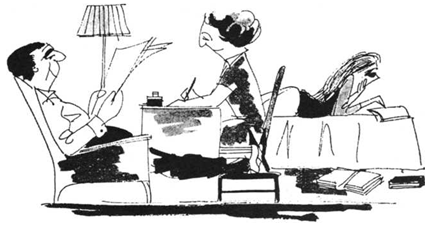
\includegraphics{img/L02.png}
\end{center}

Isa on täna kodus. Ta istub ja loeb. Ema on ka siin. Ta kirjutab. Tütar õpib. Poeg tuleb ja küsib: \guillemotleft Mis te siin teete?\guillemotright Õde vastab: \guillemotleft Armas vend, sa näed ju ise: me istume, õpime, loeme ja kirjutame.\guillemotright\\

% =======================
% 		VOCABULARIO
% =======================
\Large{\section*{Vocabulario}}

\begin{tabular}{ l l }
	aga				& pero \\
	armas			& querido/a \\
	ema				& madre \\
	hallo			& hola \\
	isa				& padre \\
	ise				& mismo (yo mismo, tú mismo, etc.) \\
	istu/n			& (yo) me siento  \\
	jah				& sí \\
	ju				& por supuesto \\
	kas				& interrogación \\
	kes				& quién \\
	kuid			& aunque, pero \\
	kuidas			& cómo \\
	kuidas läheb?	& ¿cómo va? \\
	kus				& dónde \\
	küll			& ciertamente \\
	küsi/n			& (yo) pregunto \\
	laud			& mesa, pizarra \\
	loe/n			& (yo) leo \\
	lähe/n			& (yo) voy \\
	mis				& qué \\
	näe/n			& (yo) veo \\
	poeg			& hijo \\
	poiss			& niño \\
	see				& esto \\
	seisa/n			& (yo) me paro \\
	tea/n			& (yo) sé \\
	tee/n			& (yo) hago \\
	tool			& silla \\
	tore			& bien, fabuloso, divertido \\
	tüdruk			& niña \\
	tütar			& hija \\
	vasta/n			& (yo) respondo \\
	vend			& hermano \\
	õde				& hermana
\end{tabular}

% ======================
% 		EJERCICIOS
% ======================
\Large{\section*{Ejercicios}}

\begin{enumerate}
	\item \emph{Conjugue los siguientes verbos en estonio en tiempo presente:} hacer, saber, preguntar, responder, sentarse, pararse.
	\item \emph{Traducir al estonio:} ¿Dónde vives? ¿Quién está preguntando? ¿Estás en casa? ¿Dónde están? ¿Qué están haciendo aquí? Estamos sentados y hablando. ¿Está el niño parado? Sí, él está parado aquí. ¿Qué está haciendo la niña? La niña está sentada y leyendo. ¿Qué es esto? ¿Ustedes saben? ¿Tú sabes qué es esto? El hermano está aquí, pero la hermana está ahí. ¿Dónde está papá? ¿Qué está haciendo mamá? Yo voy a preguntar, y tú vas a responder. ¡Por favor (acepte esto)! ¡Muchas gracias!
	\item \emph{Traduzca al español:} Kas sa tuled homme? Kes seal on? Kus sa elad? Kuidas läheb? Mis see on? 
\end{enumerate}

% ============================
% 		EXPRESIONES DE ...
% ============================
\Large{\section*{Expresiones de preocupación}}

\begin{tabular}{ l p{6.5cm} }
	Kuidas käsi käib?				& ¿Cómo estás? (\emph{lit.} ¿Cómo va la mano?) \\
	Kuidas läheb?					& ¿Cómo va? \\
	Kuidas elad? Kuidas elate?		& ¿Cómo te sientes? (\emph{lit.} ¿Cómo estás/está viviendo?) \\
	Tänan, hästi.					& Bien, gracias. \\
	Kuidas ise elate?				& ¿Cómo se siente usted? \\
	Suur tänu, kõik on hästi.		& Muchas gracias, todo está bien. (\emph{lit.} Grande gracias, todo está bien.) \\
	Aitäh, pole viga.				& Gracias, no hay problemas. \\
	Halvasti.						& Mal. \\
	Mis sa soovid? Mida te soovite? & ¿Qué deseas? ¿Qué desean? \\
	Kas te soovite (midagi)?		& ¿Desean algo? \\
	Jah, palun. Ei, tänan.			& Sí, por favor. No, gracias. \\
	Kas jah või ei?					& ¿Sí o no?
\end{tabular}

% ======================================
% 		RESPUESTA A LOS EJERCICIOS
% ======================================
\Large{\section*{Respuesta a los ejercicios}}

\begin{enumerate}
\item
\begin{tabular}{ l l l l l l l }
(ma)	& teen		& tean		& küsin		& vastan	& istun		& seisan \\
(sa)	& teed		& tead		& küsid		& vastad	& istud		& seisad \\
(ta)	& teeb		& teab		& küsib		& vastab	& istub		& seisab \\
(me)	& teeme		& teame		& küsime	& vastame	& istume	& seisame \\
(te)	& teete		& teate		& küsite	& vastate	& istute	& seisate \\
(nad)	& teevad	& teavad	& küsivad	& vastavad	& istuvad	& seisavad
\end{tabular}
\item Kus sa elad? Kes küsib? Kas (sa) oled kodus? [= Oled (sa) kodus?] Kus nad on? Mis te siin teete? [= Mis te teete siin?] Me istume ja räägime. Kas poiss seisab? Jah, ta seisab siin. Mis tüdruk teeb? [= Mis teeb tüdruk?] Tüdruk istub ja loeb. Mis see on? Kas (te) teate? Kas sa tead, mis see on? Vend on siin, aga [= kuid] õde on seal. Kus isa on? Mis ema teeb? Mina küsin, ja sina vastad. Palun! Tänan väga!
\item ¿Vienes mañana? ¿Quién está ahí? ¿Dónde vives? ¿Cómo va? ¿Qué es esto?
\end{enumerate}
%----------------------------------------------------------------------------------------
% ======================================
%
% 				Lesson 3
%
% ======================================

\chapter{Tercera Lección} 

\label{ch:lesson03} 

%----------------------------------------------------------------------------------------

% =====================
% 		GRAMATICA
% =====================
\Large{\section*{Gramática}}

\S\ 14. La raíz del tiempo presente de un verbo, carente de terminaciones (por ejemplo, \textbf{tule-} \textless\ tule/n, \textbf{loe-} \textless\ loe/n, \textbf{räägi-} \textless\ räägi/n), puede ser utilizada de las siguientes maneras:

\begin{itemize}
	\item como la forma imperativa (ordenes) para la segunda persona singular

	\begin{center}
	\begin{tabular}{ l l }
		\textbf{tule!}	& ¡ven! \\
		\textbf{loe!}	& ¡lee! \\
		\textbf{räägi!}	& ¡habla!
	\end{tabular}	
	\end{center}
	\bigskip

	en la forma negativa

	\begin{center}
	\begin{tabular}{ l l }
		\textbf{ära tule!}	& ¡no vengas! \\
		\textbf{ära loe!}	& ¡no leas! \\
		\textbf{ära räägi!}	& ¡no hables!
	\end{tabular}	
	\end{center}
	\bigskip

	Nota: El imperativo del verbo lähe/n `ir' se obtiene de otra raíz: \textbf{mine!} `ve', \textbf{ära mine!} `no vayas!'

	\S\ 15. 

	\item como la forma en tiempo presente negativo con la partícula negativa \textbf{ei}, que siempre se coloca delante del verbo. Esta construcción se utiliza para todas las personas en singular y plural.

	\begin{center}
	\begin{tabular}{ l l }
		mina \textbf{ei tule}	& yo no voy a venir \\
		sina \textbf{ei tule}	& tú no vas a venir \\
		tema \textbf{ei tule}	& él/ella no va a venir \\
		& \\
		meie \textbf{ei tule}	& nosotros no vamos a venir \\
		teie \textbf{ei tule}	& ustedes no van a venir \\
		nemad \textbf{ei tule}	& ellos/ellas no van a venir
	\end{tabular}	
	\end{center}	
	\bigskip
\end{itemize}

\S\ 16. La partícula negativa extra \textbf{mitte} puede ser usado para fortalecer el tono de una negación común. 

\begin{center}
\begin{tabular}{ l l }
	ma \textbf{ei tule mitte!} & ¡yo \emph{no} voy a venir!
\end{tabular}	
\end{center}
\bigskip

Observe que la partícula negativa ordinaria \textbf{ei} debe ser incluida.

\S\ 17. Como una forma alternativa para \textbf{ei ole} `no soy/eres/es/somos/son/son/estoy/estas/está/estamos/están/están', la palabra \textbf{pole} se utiliza a menudo, con el mismo significado. (Esta es una contracción de \textbf{ep+ole}, donde \textbf{ep} es una forma arcaica de la partícula negativa \textbf{ei}).

\begin{center}
\begin{tabular}{ l l }
	ta \textbf{ei ole} siin = ta \textbf{pole} siin & `él/ella no está aquí' \\
	ma \textbf{ei ole} valmis = ma \textbf{pole} valmis & `yo no estoy listo' 
\end{tabular}	
\end{center}
\bigskip

\S\ 18. Una respuesta negativa a una pregunta a menudo consiste en la partícula negativa \textbf{ei} con el verbo en cuestión.

\begin{center}
\begin{tabular}{ l l }
	Kas sa \textbf{oled} kodus? & `¿Estás tú en casa?' \\
	\textbf{Ei ole} & `No estoy' \\
	& \\
	Kas te \textbf{tulete}? & `¿Vienen ustedes?' \\
	\textbf{Ei tule} & `No vamos' \\
\end{tabular}	
\end{center}
\bigskip

\S\ 19. El estonio tiene muchos verbos con partículas adverbiales, que corresponden a frases en inglés como `get up', `go out', y similares. Por ejemplo: \textbf{tõusen üles} `me levanto', \textbf{tõusen püsti} `me pongo de pie', \textbf{saan aru} `entiendo' [\emph{lit.}: `adquiero inteligencia'], \textbf{vaatan pealt} `parezco'.\\

En estas situaciones, sólo el verbo cambia en el proceso de conjugación. La partícula acompañante se mantiene sin cambios.

\begin{center}
\begin{tabular}{ l l l l }
	ma \textbf{saan aru} & `yo entiendo' 		& me \textbf{saame aru} `nosotros entendemos' \\
	sa \textbf{saad aru} & `tú entiendes'		& te \textbf{saate aru}	`ustedes entienden' \\
	ta \textbf{saab aru} & `él/ella entiende' 	& nad \textbf{saavad aru} `ellos entienden'
\end{tabular}	
\end{center}
\bigskip

La partícula puede ser separada del verbo por otras partes de la oración. Por ejemplo: ma \textbf{tõusen} kohe \textbf{püsti} `Me levantaré inmediatamente', ma \textbf{saan} hasti \textbf{aru} `Yo entiendo bien'.


% ==================
% 		TEXTO
% ==================
\Large{\section*{Texto}}

Tule siia! Palun, istu. Jutusta, ma kuulan. Räägi kõvasti. Ära räägi nii tasa! Ma ei saa aru, mis sa ütled. Ma ei kuule hästi. Ma kuulen halvasti.\\
Ütle, mis see on! Ma ei tea, mis see on. Vaata, kes seal seisab! Kas sa näed? Ei, ma ei näe. Ma lähen kohe ja vaatan. Mine sinna ja küsi! Tule siia tagasi!\\
Enne mõtle, siis ütle!\\

Kuhu sa lähed, armas sõber? Lähen koju. Perekond on kodus ja ootab. Oota, ma tulen ka kohe! Poeg on kodus. Tütar ei ole. Ta pole veel kodus.\\
Kas te õpite? Ei, me ei õpi. Me lamame ja puhkame. Kas te seisate, või istute? Vend seisab, aga õde istub. Palun vasta, kui ma küsin! Tõuse püsti, kui sa räägid! Kas sa saad aru, mis ma ütlen? Ma kardan, et ma ei saa hästi aru. Kas sa tead, mis seal on? Ma tõesti ei tea.

% =======================
% 		VOCABULARIO
% =======================
\Large{\section*{Vocabulario}}

\begin{tabular}{ l l }
	aru				& entendimiento \\
	ei				& no \\
	enne			& antes, primero \\
	et				& que [\emph{conj.}] \\
	halvasti		& mal \\
	jutusta/n		& (yo) narro \\
	karda/n			& (yo) temo \\
	kodus			& en casa \\
	kohe			& inmediatamente \\
	koju			& a casa \\
	kuhu			& a dónde, adonde \\
	kui				& cuando, si, como \\
	kuula/n			& (yo) escucho \\
	kuule/n			& (yo) oigo \\
	kõvasti			& fuerte, ruidoso \\
	lama/n			& (yo) me reclino \\
	mine			& anda! \\
	mõtle/n			& (yo) pienso \\ 
	nii				& entonces [\emph{adj.}] \\
	oota/n			& (yo) espero \\ 
	perekond		& familia \\
	pole = ei ole	& no soy/eres/es ... \\
	puhka/n			& (yo) descanso \\
	saa/n aru		& (yo) entiendo \\ 
	siia			& hacia aquí \\
	siis 			& entonces \\	
	sinna			& hacia allá \\ 
	sõber			& amigo  \\
	tagasi			& atrás [\emph{adv.}] \\
	tasa			& despacio \\
	tõesti			& verdaderamente \\
	tõusen			& (yo) me levando \\
	tõusen püsti	& (yo) me paro \\
	vaata/n			& (yo) miro \\
	veel			& todavía, más \\
	või				& o \\
	ära				& no \\
	ütle/n			& (yo) digo
\end{tabular}

% ======================
% 		EJERCICIOS
% ======================
\Large{\section*{Ejercicios}}

\begin{enumerate}
	\item \emph{Traduzca al estonio:} Yo esperaré aquí. Tú hablas fuerte, pero él habla despacio. Ellos entienden. Ustedes narran bien. Yo digo que vamos a venir de inmediato. ¿Vendrás de inmediato?\\

	Ellos vienen aquí. Nosotros vamos hacia allá. ¡Ven aquí! ¡Ve allí! Lo veré por mi mismo. Él oye muy bien. ¡Vuelve inmediatamente!. ¡Espera aquí! ¡Habla en voz alta! ¡No hables tan alto! ¿Están de pie o sentados? Di, ¿vas a venir mañana? No, no voy a venir.

	\item \emph{Traduzca al español:} Ma kuulen. Ta kuulab. Sa näed. Me vaatame. Te räägite. Nad ütlevad. Olen kodus. Ta läheb koju. Mina olen siin. Tule ka siia! Nemad on seal. Mine sinna!
\end{enumerate}

% ============================
% 		EXPRESIONES DE ...
% ============================
\Large{\section*{Expresiones de Cortesía}}

\begin{tabular}{ l l }
	\textbf{Kas ma segan?}				& ¿Estoy molestando? \\
	\textbf{Ei, mitte sugugi!}			& No, en absoluto! \\
	\textbf{Pole viga.}					& No hay problema. \\
	\textbf{Ei, sa/te ei sega.}			& No, no me estás molestando. \\
	\textbf{Astu sisse!}				& ¡Adelante! \\
	\textbf{Astuge sisse, palun!}		& ¡Adelante, por favor! \\
	\textbf{Tule siia! Tulge siia!}		& ¡Ven aquí!, ¡Venga aquí! \\
	\textbf{Palun, istu/istuge!}		& Por favor, siéntate/siéntese. \\
	\textbf{Vabanda! Vabandage!}		& ¡Disculpa! ¡Disculpe! \\
	\textbf{Palun vabandust! Vabandust!}& ¡Le pido (su) perdón! ¡Perdón! \\
	\textbf{Vabandage, et tülitan.}		& Perdone por molestar. \\
	\textbf{Palun väga!}				& Por favor (aceptar esto). \\
	\textbf{(Oota) üks silmapilk!}		& (Espere) un momento. \\
	\textbf{Räägi, ma kuulen.}			& Hable, yo escucho. \\
	\textbf{Ära räägi! Kas tõesti?}		& ¡No me digas! ¿En serio?
\end{tabular}

% ======================================
% 		RESPUESTA A LOS EJERCICIOS
% ======================================
\Large{\section*{\Large{Respuesta a los ejercicios}}

\begin{enumerate}
	\item Mina [= ma] ootan siin. Sina räägid kõvasti, aga tema räägib tasa. Nemad saavad aru. Teie jutustate hästi. Ma ütlen, et me tuleme kohe. (Kas sa) tuled kohe?\\

	Nemad tulevad siia. Meie läheme sinna. Tule siia! Mine sinna! Ma näen ise. Ta kuuleb väga hästi. Tule kohe tagasi! Oota siin! Räägi 	kõvasti! Ära räägi nii kõvasti! Kas te seisate või istute? Ütle, kas sa tuled homme? Ei, ma ei tule mitte.

	\item  Yo oigo. Él/ella escucha. Tú ves. Nos miramos. Ustedes hablan. Ellos dicen. Estoy en casa. Él/ella se va a casa. Estoy aquí. ¡Ven hacia aquí también! Ellos están ahí. ¡Ve allí!
\end{enumerate}
%---------------------------------------------------------------------------------------- 
% Lesson 4

\chapter{Cuarta Lección} % Chapter title

\label{ch:lesson04} % For referencing the chapter elsewhere, use \autoref{ch:examples} 

%----------------------------------------------------------------------------------------

% =====================
% 		GRAMATICA
% =====================
\Large{\section*{Gramática}}

\bemph{\subsection*{Caso Nominativo Singular}}

\S\ 20. La forma del caso nominativo de ambos sustantivos y adjetivos no tiene una terminación en particular. Puede terminar en casi cualquier vocal o consonante.\\

\begin{center}
\begin{tabular}{ l }
	 \bemph{isa} `padre', \bemph{õde} `hermana', \bemph{käsi} `mano', \bemph{töö} `trabajo', \\ 
	 \bemph{vana} `viejo/vieja', \bemph{terve} `saludable', \bemph{hea} `bien', \bemph{mees} `hombre', \\
	 \bemph{sõber} `amigo', \bemph{raamat} `libro', \bemph{noor} `joven', \bemph{paks} `gordo/gorda', \\
	 \bemph{kõhn} `delgado/delgada', \bemph{vend} `hermano', \bemph{laps} `niño/niña'
\end{tabular}
\end{center}
\bigskip

\S\ 21. El caso nominativo (\bemph{nimetav kääne} en estonio) responde a las preguntas \bemph{kes?} `¿quién?', \bemph{mis?} `¿qué?', \bemph{milline?} (o \bemph{missugune?}) `¿qué tipo?'. Se utiliza principalmente para los sujetos de las oraciones y los complementos del predicado.\\

\begin{center}
\begin{tabular}{ l l }
	\bemph{Kes} kirjutab?	&	`¿Quién escribe?' \\
	\bemph{Vend} kirjutab.	&	`El hermano escribe.' \\
	&  \\		
	\bemph{Kes} ta on?		&	`¿Quién es él/ella?' \\
	Ta on \bemph{õpetaja}.	&	`Él/Ella es un/una profesor/profesora.' \\
	&  \\	
	\bemph{Milline} ta on?	&	`¿Qué tipo es él/ella?' (¿Cómo es él/ella?)' \\
	Ta on \bemph{noor}.		&	`Él/Ella es joven.' \\
	&  \\
	\bemph{Mis} seal on?	&	`¿Qué es eso?' \\
	Seal on \bemph{laud}.	&	`Eso es una mesa.' \\
	&  \\
	\bemph{Mis} see on?		&	`¿Qué es eso?' \\
	See on \bemph{raamat}.	&	`Eso es un libro.' 
\end{tabular}
\end{center}
\bigskip

\S\ 22. Al igual que en español, el verbo se conjuga de acuerdo al pronombre personal y no a la palabra `Ese' en las cláusulas del tipo `Ese soy yo'. \\

\begin{center}
See \bemph{olen mina}. `Ese soy yo.' See \bemph{oled sina}. `Ese eres tú.' See \bemph{on tema}. `Ese es él/ella.'
\end{center}

\S\ 23. En una oración negativa, se usa a menudo una doble negación. El español no tiene tal partícula, pero equivaldría a recalcar la partícula negativa de la oración. Esto quiere decir que en el estonio la doble negación sigue siendo negativa, utilizando la partícula \bemph{mitte} para reforzar el impacto negativo del \bemph{ei}.\\

\begin{center}
\begin{tabular}{ l l }
	Ma \bemph{ei} tea \bemph{mitte midagi}.			& `Yo no sé \bemph{nada}.' \\
	&  \\
	Ta \bemph{ei} tule \bemph{mitte iialgi} tagasi. & `Él/Ella \bemph{nunca} volverá.'
\end{tabular}
\end{center}
\bigskip

% ==================
% 		TEXTO
% ==================
\Large{\section*{Texto}}

Vend on juba suur poiss. Ta käib koolis. Õde on väike tüdruk. Ta mängib kodus. Ta on hea laps. Vanaisa ja vanaema istuvad ja puhkavad. Nad vaatavad pealt kuidas väike laps mängib. Tädi ja onu tulevad homme külla. Siis on ka vanemad kodus.\\
Kas isa on vana mees? Ei ole, isa on veel noor inimene. Ema on ka noor. Ema on noor naine. Onu on aga juba vana mees. Milline on tädi? Tädi on noor ja ilus. \\

\begin{center}
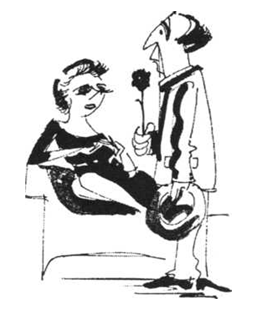
\includegraphics{img/L04.png}
\end{center}
\bigskip

\noindent
-- Mida te teete, proua Kivisaar, et te nii noor ja ilus välja näete? \\
-- Ma ei tee mitte midagi. \\

\noindent
Rumal räägib, mis ta teab, tark teab, mis ta räägib. \\
Kõik pole kuld, mis hiilgab, (Vanasõna) \\
Üles läheb, alla ei tule. (Mõistatus) -- Suits. \\

% =======================
% 		VOCABULARIO
% =======================
\Large{\section*{Vocabulario}}

\begin{tabular}{ l l }
alla			&	abajo \\
hea				&	bien, bueno \\
hiilga/n		&	(Yo) brillo \\
ilus			&	hermosa, linda \\
inimene			&	persona \\
juba			&	ya (\eg ya estoy listo) \\
koolis			&	en el colegio  \\
kuld			&	oro \\
kõik			&	todo \\
käi/n koolis	&	(Yo) voy al colegio \\
külla			&	de visita \\
laps			&	niño/niña \\
mees			&	hombre \\
mida [= mis]	&	qué \\
midagi			&	algo, nada \\
milline			&	qué tipo \\
mitte			&	(reforzador de negación) \\
mitte midagi	&	(absolutamente) nada \\
mõistatus		&	acertijo  \\
mängi/n			&	(Yo) juego \\
naine			&	mujer \\
noor			&	joven \\
näe/n välia		&	(Yo) parezco, Me veo \\
onu				&	tío \\
proua			&	Sra. (Señora) \\
rumal			&	(persona) estúpida  \\
suits			&	humo \\
suur			&	grande \\
tark			&	(persona) astuta, inteligente  \\
tädi			&	tía \\
vaata/n pealt	&	(Yo) observo \\
vana			&	viejo/vieja \\
vanaema			&	abuela \\
vanaisa			&	abuelo \\
vanasõna		&	proverbio, dicho antiguo \\
vanemad			&	padres, ancianos \\
väike			&	pequeño \\
üles			&	arriba
\end{tabular}
\bigskip

% ======================
% 		EJERCICIOS
% ======================
\Large{\section*{Ejercicios}}

\begin{enumerate}
	\item \emph{Traducir al estonio:} ¿Qué es esto? Este es una tabla. ¿Quién está allí? Soy Yo. ¿Quién va a la escuela? Él es un buen chico. ¿La pequeña hermana también va a la escuela? No, ella no va a la escuela todavía. Ella es una niña. Hermano y hermana juegan en casa. ¿Van ustedes a casa? Vamos a estar en casa mañana. El abuelo es un hombre viejo. La sra. Kivisaar es una mujer joven. Ella es muy bonita. ¿El tío es joven? No, no es joven, ya es viejo. ¿Es muy viejo? No, no lo es. ¿Qué está haciendo la tía hoy? No sé. ¿Entiendes lo que digo? ¡Di algo! ¡No hables en voz tan baja!

	\item \emph{Traducir al español:} 

	\begin{center}
	\begin{tabular}{ l l }
		mees -- naine		& poeg -- tütar \\  
		poiss -- tüdruk   	& vend — õde \\ 
		isa -- ema 			& onu -- tädi \\
		vanaisa — vanaema	& laps -- vanemad - perekond
	\end{tabular}
	\end{center}
	\bigskip
\end{enumerate}

% ============================
% 		EXPRESIONES DE ...
% ============================
\Large{\section*{Expresiones de Curiosidad}}

\begin{tabular}{ l l }
	Mis see on?							& ¿Qué es esto? \\
	Mis see tähendab?					& ¿Qué significa esto? \\
	Kes seal on? Kes see on? 			& ¿Quién está allí? ¿Quién es (este)? \\
	See on härra/proua/preili... 		& (Este) es el/la señor/señora/señorita ...\\
	Kas see on proua Palm?				& ¿Es (esta) la señora Palm? \\
	Jah, on küll. -- E¡ ole.			& Sí, lo es. -- No lo es. \\
	Kuidas te teate?					& ¿Cómo saben? \\
	Mis sa arvad? Mis te arvate?		& ¿Qué crees tú? ¿Qué creen ustedes? \\
	Kas sa saad aru? Kas te saate aru? 	& ¿Entiendes? ¿Entienden? \\
	Saan aru. -- Ma ei saa aru.			& Entiendo -- No entiendo \\
	Kuidas, palun?						& ¿Disculpa? (¿qué dijiste?) \\
	Vabandust, ma ei kuulnud.			& Perdón, no escuché. \\
	Palun korda! Palun korrake!			& ¡Por favor repite! ¡Por favor repita!  
\end{tabular}
\bigskip

% ======================================
% 		RESPUESTA A LOS EJERCICIOS
% ======================================
\Large{\section*{Respuesta a los ejercicios}}

\begin{enumerate}
	\item Mis see on? See on (üks) laud. Kes seisab seal? See olen mina. Kes käib koolis? Ta on hea poiss. Kas väike õde käib ka koolis? Ei, tema ei käi veel koolis. Ta on väike tüdruk. Vend ja õde mängivad kodus. Kas te lähete koju? Me oleme homme kodus. Vanaisa on vana mees. Proua Kivisaar on noor naine. Ta on väga ilus. Kas onu on noor inimene? Ei, ta pole [= ei ole] noor, ta on vana. Kas ta on väga vana? Ei ole. Mis tädi teeb täna? Ma ei tea. Kas sa saad aru, mis ma ütlen? Ütle midagi! Ära räägi nii tasa!

	\item 
	\begin{tabular}{ l l }
		hombre -- mujer		& hijo -- hija \\
		niño -- niña		& hermano -- hermana \\
		padre -- madre		& tío -- tía \\
		abuelo -- abuela	& laps -- vanemad -- perekond 
	\end{tabular}
\end{enumerate}

%----------------------------------------------------------------------------------------
% Lesson 5

\chapter{Quinta Lección} % Chapter title

\label{ch:lesson05} % For referencing the chapter elsewhere, use \autoref{ch:examples} 

%----------------------------------------------------------------------------------------


% =====================
% 		GRAMATICA
% =====================
\Large{\section*{Gramática}}

\S\ 24. Después de una orden, el llamado objeto definido u objeto total se encuentra en el caso nominativo. Un objeto es "total" si el mismo  está implicado en la acción (véase el \autoref{ch:lesson28}). Ejemplos:

\begin{center}
\begin{tabular}{ l l }
	Too \bemph{raama}t siia!		&	`¡Trae el libro (aquí)!' \\
	Vii \bemph{laps} koju!			&	`¡Lleva al niño a casa!' \\
	Kutsu \bemph{vend} siia!		&	`¡Llama al hermano aquí!' \\
	Anna mulle \bemph{üks dollar}!	&	`¡Dame (a mí) un dolar!' \\
	Võta see \bemph{ajaleht}!		&	`¡Toma ese periódico!' 
\end{tabular}
\end{center}
\bigskip

\S\ 25. Construcciones impersonales del tipo `está caluroso' se expresan en estonio sólo por el verbo en tercera persona del singular, al igual que en español. \\

\begin{center}
\begin{tabular}{ l l }
	\bemph{On} võimaik, et ...		&	`Es posible que ...' \\
	Täna \bemph{on} ilus ilm.		&	`Hoy es un día hermoso.' \\
	Toas \bemph{on} soe.			&	`En la habitación está caluroso.' \\
	Kuidas \bemph{läheb}?			&	`¿Cómo estás?' [\emph{lit.:} ¿Cómo va?] \\
	\bemph{Sajab}.					&	`Llueve.' \\
	Mind \bemph{huvitab}, kas ...	&	`Me interesa, que ...' 
\end{tabular}
\end{center}
\bigskip

En ciertos casos, incluso el verbo puede omitirse: \\

\begin{center}
\begin{tabular}{ l l }
	Väga \bemph{võimalik}, et ...	& `Es muy probable que ...' \\
	\bemph{Huvitav}, kas ...		& `Sería interesante que ...' \\
	\bemph{Imelik}, et ...			& `Es extraño que ...'
\end{tabular}
\end{center}
\bigskip

\S\ 26. Números 0 - 10 \\

\begin{center}
\begin{tabular}{ l c l }
	0	null	& &	6 kuus \\
	1	üks		& &	7 seitse \\
	2	kaks	& &	8 kaheksa \\
	3	kolm	& &	9 üheksa \\
	4	neli	& &	10 kümme \\
	5	viis	& & 
\end{tabular}
\end{center}
\bigskip

% ==================
% 		TEXTO
% ==================
\Large{\section*{Texto}}

Võta raamat ja tule siia. Ava raamat ja loe! Kas see on huvitav raamat? See on õpik! \\
Võta see sulepea ja kirjuta. Kirjuta üks kiri! Saada kiri isale. Anna sulepea mulle tagasi. \\

Ole hea, too pliiats siia! Võta pliiats ja joonista. Joonista üks pilt. See on ilus pilt! Kingi see pilt mulle! \\

Osta homme uus õpik. Too õpik kaasa, kui sa tuled. Kutsu sõber ka kaasa. Huvitav, kas ta tuleb? Kui on halb ilm, siis istume toas ja õpime. Kui aga ilm on ilus, siis läheme jalutama. \\
Täna sa töötad, aga homme puhkad. Sa õpid hästi, sa oled hea õpilane. Tänan, kuid teie õpetate hästi. Te olete hea õpetaja. \\
Väike tüdruk laulab. See on väga ilus laul. Laula veel üks laul! \\

Kui palju on seitse ja kolm? Seitse ja kolm on kümme. Kui palju on kaks ja viis? Kaks ja viis on seitse. Kui palju on üks pluss neli? Üks pluss neli on viis. Üheksa miinus kuus on kolm. \\

\noindent
-- Ütle, palun, mis arv see on: 5? \\
-- See on viis. \\
-- Õige! Aga mis arv see on: 7? \\
-- Kaheksa? \\ 
-- Vale! See on seitse. Õpi veel! \\

\begin{center}
Üheksa korda mõtle, üks kord ütle. (Vanasõna)
\end{center}

% =======================
% 		VOCABULARIO
% =======================
\Large{\section*{Vocabulario}}

\begin{tabular}{ l l }
anna/n		&	(Yo) doy \\
arv			&	número \\
ava/n		&	(Yo) abro \\
halb		&	malo \\
huvitav		&	interesante \\
ilm			&	tiempo, clima \\
isale		&	al padre \\
jaluta/n	&	(Yo) camino, paseo \\
joonista/n	&	(Yo) dibujo \\
kaasa		&	consigo \\
kingi/n		&	(Yo) regalo \\
kiri		&	carta \\
kord		&	vez, ocasión \\
korda		&	veces, ocasiones \\
kui palju	&	Cuánto \\
kutsu/n		&	(Yo) invito, llamo \\
laul		&	canción \\
laula/n		&	(Yo) canto \\
miinus		&	menos \\
mulle		&	para mí \\
osta/n		&	(Yo) compro \\
palju		&	mucho \\
pilt		&	imagen, fotografía \\
pliiats		&	lápiz \\
pluss		&	más, suma \\
raamat		&	libro \\
saada/n		&	(Yo) envío \\
sulepea		&	pluma (para escribir) \\
toas		&	en la habitación \\
too/n		&	(Yo) traigo, llevo \\
tööta/n		&	(Yo) trabajo \\
uus			& 	nuevo \\
vale		&	incorrecto, malo \\
võta/n		&	(Yo) tomo \\
õige		&	correcto, bien \\
õpetaja		&	profesor \\
õpeta/n		&	(Yo) enseño \\
õpik		&	manual \\
õpilane		&	estudiante
\end{tabular}
\bigskip

% ======================
% 		EJERCICIOS
% ======================
\Large{\section*{Ejercicios}}

\begin{enumerate}
	\item \emph{Traducir al estonio:} El padre es un profesor. El maestro enseña. El hijo es un estudiante. El estudiante estudia. ¡Dame este libro! Por favor, abre el libro. Canta una canción. Hay buen tiempo hoy. No voy a hacer nada hoy. Descansaremos hoy, pero mañana vamos a trabajar. ¿A dónde van? Estamos caminando a casa. Compra un nuevo libro. Lleva el libro contigo, cuando vengas.

	\item \emph{Diga en estonio:} ¿Cuánto es dos y cuatro? 1+9 = 10, 2+6 = 8, 3+4 = 7, 5+5 = 10, 8-7 = 1, 9-6 = 3, 2-2 = 0, 6-5 = 1.

	\item \emph{Traduzca las siguientes frases al español:} \\
		\begin{tabular}{ l l }
			tõusen püsti 	& saad aru \\
			vaatame pealt 	& näete välja  
		\end{tabular}

	\item \emph{Traduzca las siguientes frases al español:} Poiss \bemph{ja} tüdruk. Suur \bemph{või} väike? \bemph{Kas} jah \bemph{või} ei? Ma näen, \bemph{et} ... Tüdruk istub, \bemph{aga} poiss seisab. See on \bemph{nii} ilus! Õde ei ole \bemph{nii} suur \bemph{kui} vend.\bemph{Kui} sa tuled, võta sõber \bemph{ka} kaasa!
\end{enumerate}

% ============================
% 		EXPRESIONES DE ...
% ============================
\Large{\section*{Expresiones de Evaluación}}

\begin{tabular}{ l l }
	\bemph{Kas sa oled rahul?}						& ¿Estás satisfecho? [\emph{lit.:} en paz] \\
	\bemph{Jah, täiesti!}							& Sí, completamente. \\
	\bemph{Suur [= Palju] tänu, kõik on korras.}	& Muchas gracias, todo está en orden. \\
	\bemph{On(s) see tõsi?}							& ¿Es cierto? \\
	\bemph{See on sulatõsi!}						& ¡Es la pura verdad! \\
	\bemph{See on puha vale!}						& ¡Es una mentira! \\
	\bemph{Sa eksid! Te eksite!}					& ¡Te equivocas! ¡Se equivoca (usted)! \\
	\bemph{Laula üks laul!}							& ¡Canta una canción! \\
	\bemph{Ma ei oska.}								& No puedo. (No sé cómo.) \\
	\bemph{Ah nii?!}								& ¡¿Ah, sí?! 
\end{tabular}

% ======================================
% 		RESPUESTA A LOS EJERCICIOS
% ======================================
\Large{\section*{Respuesta a los ejercicios}}

\begin{enumerate}
	\item Isa on õpetaja. Õpetaja õpetab. Poeg on õpilane. Õpilane õpib. Anna mulle see raamat! Palun [= Ole hea], ava raamat! Laula üks laul! Täna on ilus ilm. Ma ei tee täna mitte midagi. Täna me puhkame, aga [= kuid] homme me töötame. Kuhu te lähete? Me jalutame koju. Osta (üks) uus raamat. Too raamat kaasa, kui (sa) tuled.

	\item Kui palju on kaks ja neli? Üks ja [= pluss] üheksa on kümme, kaks ja kuus on kaheksa, kolm ja neli on seitse, viis ja viis on kümme, kaheksa miinus seitse on üks, üheksa miinus kuus on kolm, kaks miinus kaks on null, kuus miinus viis on üks

	\item 
		\begin{tabular}{ l l }
			Me levanto 			& tú entiendes \\
			miramos, observamos & ustedes parecen, se ven como  
		\end{tabular}

	\item Un niño y una niña. ¿Grande o pequeño? ¿Sí o no? Veo que ... La niña está sentada, pero el niño está parado. ¡Esto es tan hermoso! La hermana no es tan grande como el hermano. Cuando vengas, ¡trae al amigo contigo también!.
\end{enumerate}

%----------------------------------------------------------------------------------------
% Lesson 6

\chapter{Sexta Lección} % Chapter title

\label{ch:lesson06} % For referencing the chapter elsewhere, use \autoref{ch:examples} 

%----------------------------------------------------------------------------------------


% =====================
% 		GRAMATICA
% =====================
\Large{\section*{Gramática}}

\bemph{\subsection*{Tiempo Presente Condicional}}

\S\ 27. El presente condicional, que corresponde a las expresiones con terminación `-ría' en español, se construye en el estonio con la raíz del tiempo presente, seguido de \bemph{-ksi-} y la terminación final en tiempo presente en la primera y segunda persona singular/plural. La tercera persona del singular/plural no sigue este patrón. \\

\begin{tabular}{ l l l }
	 					& \emph{Presente} 					& \emph{Presente Condicional} \\
	\emph{Singular} 	& 1. ma \bemph{taha/n} `Yo quiero' 	& \bemph{taha/ksi/n} `Yo querría' \\
	 					& 2. sa \bemph{taha/d} 				& \bemph{taha/ksi/d} \\
	 					& 3. ta \bemph{taha/b} 				& \bemph{taha/ks/-} \\
	 					& & \\
	\emph{Plural} 		& 1. me \bemph{taha/me} 			& \bemph{taha/ksi/me} \\
	 					& 2. te \bemph{taha/te} 			& \bemph{taha/ksi/te} \\
	 					& 3. nad \bemph{taha/vad} 			& \bemph{taha/ksi/d}
\end{tabular}
\bigskip

Ejemplo: Ma tahaksin minna koju. `Querría (Me gustaría) ir a casa.' \\

\S\ 28. La forma negativa del condicional consiste en \bemph{ei + tercera persona singular} del verbo, para todas las personas. \\

\begin{tabular}{ l l }
	ma \bemph{ei tahaks} `Yo no querría' 	& me \bemph{ei tahaks} \\
	sa \bemph{ei tahaks} 					& te \bemph{ei tahaks} \\
	ta \bemph{ei tahaks} 					& nad \bemph{ei tahaks}
\end{tabular}
\bigskip

Ejemplo: Me \bemph{ei tahaks} minna koju. `No querríamos (No nos gustaría) ir a casa.' \\

Nota: Esta forma es aceptada incluso en el caso afirmativo, sobre todo en estonio hablado. En este caso, el elemento negativo `ei' se descarta. \\

\begin{center}
Ma \bemph{tahaks} [en vez de \bemph{tahaksin}] minna koju. \\
`Querría (Me gustaría) ir a casa.'
\end{center}
\bigskip

\S\ 29. En resumen, la raíz presente del verbo se utiliza para construir tanto las formas positivas como negativas de: \\

\begin{enumerate}
	\item el tiempo presente (ver \autoref{ch:lesson01})
	\item el imperativo para la segunda persona singular (ver \autoref{ch:lesson02})
	\item el tiempo condicional
\end{enumerate}
\bigskip

Por ejemplo: \\

\begin{tabular}{ l | l l }
								& \bemph{tule/n} 		& \bemph{ei tule} \\
								& `(Yo) vengo			& `(Yo) no vengo \\ 
								& & \\
	\emph{raíz del presente}	& \bemph{tule!} 		& \bemph{ära tule!} \\
	\bemph{tule-} `venir'		& `¡Ven!'				& `¡No vengas!' \\
								& & \\
								& \bemph{tule/ksi/n} 	& \bemph{ei tule/ks} \\
								& `(Yo) vendría'		& `(Yo) no vendría'
\end{tabular}
\bigskip

\S\ 30. El infinitivo (`hablar', `ir', etc. en español) a menudo tiene otra raíz que la del presente en estonio. Dado que la raíz del infinitivo es una de las formas básicas en la conjugación de un verbo en estonio (ver \autoref{ch:lesson21}), es necesario conocer tanto la raíz del infinitivo como del presente. En todos los diccionarios, el verbo siempre aparece como infinitivo (con la terminación -ma), y así será también en nuestro glosario. El infinitivo-ma es seguido por la forma en tiempo presente. Por ejemplo: \\

\begin{tabular}{ l l }
	\bemph{lugema, loe/n} 	& `leer, (Yo) leo' \\
	\bemph{lubama, luba/n} 	& `permitir, (Yo) permito' \\
	\bemph{tahtma, taha/n} 	& `querer, (Yo) quiero'
\end{tabular}

% ==================
% 		TEXTO
% ==================
\bigskip
\Large{\section*{Texto}}

Ma lähen jalutama, kui ema lubab. Ma \emph{läheksin} jalutama, kui ema \emph{lubaks}. Ma ei lähe sinna, jui sa ka lubad. Ma \emph{ei läheks} sinna, kui sa ka \emph{lubaksid}. Olen siin, kui sa tuled. \emph{Oleksin} väga rõõmus, kui sa homme siia \emph{tuleksid}. Oleks tore, kui sõber ka \emph{tuleks}. \\

Õpetaja küsib ja õpilane vastab. Kas ta oskab? Õpilane \emph{vastaks}, kui ta ainult \emph{oskaks}. Nemad istuvad, aga sina seisad. Nemad \emph{istuksid}, kui sa \emph{paluksid}. Me tahame, et te laulate. Me \emph{tahaksime}, et te \emph{laulaksite}. Kas ma tohin? Ma \emph{laulaksin}, kui ma \emph{tohiksin}. Ma \emph{tahaksin}, et sa \emph{õpiksid} hästi.	\\

Ma \emph{ei tahaks}, et sa ainult lamad ja puhkad. Sa saad, kui sa soovid. Kui sa ilusti \emph{paluksid}, siis sa \emph{saaksid}. Tee nii, nagu isa ütleb. \emph{Sooviksin}, et sa \emph{teeksid} nii, nagu ma ütlen. Nad \emph{ei teeks} nii, kui nad \emph{oleksid} kodus. \\

\begin{center}
Oleksin laululind, \\
kannaksid tiivad mind!
\end{center}
\bigskip

\noindent
Istun üksi toas. Keegi koputab. \\
-- Tee uks lahti! hüüab üks hääl. \\
-- Üks silmapilk. Tulen kohe ... Ah, sina oled! Tere! Astu sisse. Ole hea, pane uks kinni. Istu. \\
-- Tänan väga. Kas lubad, ma suitsetan? küsib sõber. \\
-- Palun väga. Luba mulle ka üks suits. \\
-- Säh, siin on karp. Võta ise üks sigarett. Siin on tikud, palun. 

% =======================
% 		VOCABULARIO
% =======================
\bigskip
\Large{\section*{Vocabulario}}

\begin{tabular}{ l l }
	ainult					& sólo [\emph{adv.}] \\
	aken					& ventana \\
	astuma, astu/n			& dar un paso, (Yo) doy un paso \\
	avatud					& abierto [\emph{adj.}] \\
	hääl					& voz \\
	hüüdma,	hüüa/n			& gritar, llamar; (Yo) grito, llamo \\
	ilusti					& bellamente, hermosamente \\
	kandma, kanna/n			& llevar, acarrear, (Yo) llevo, acarreo \\
	karp					& caja pequeña  \\
	keegi					& alguien \\
	kinni					& cerrado \\
	koputama, koputa/n		& llamar (a la puerta), (Yo) llamo a la puerta \\
	kui ... ka				& incluso si ... \\
	lahti					& abierto [\emph{adj.}] \\
	laululind				& ave cantora \\
	lind					& ave, pájaro \\
	lubama, luba/n			& permitir, (Yo) permito \\
	mind					& mí \\
	oskama, oska/n			& ser capaz, saber, (Yo) puedo \\
	pane/n kinni			& (Yo) cierro \\
	rõõmus					& feliz, contento \\
	saama, saa/n			& obtener, ser capaz; (Yo) puedo, obtengo \\
	sigarett				& cigarrillo \\
	silmapilk				& momento, `en un abrir y cerrar de ojos' \\
	sisse					& adentro  \\
	soovima, soovi/n		& desear, (Yo) deseo \\
	suits					& humo, cigarrillo \\
	suitsetama, suitseta/n	& fumar, (Yo) fumo \\
	suletud					& cerrado [\emph{adj.}] \\
	säh!					& ¡aquí tiene! ¡tome! \\
	tahtma, taha/n			& querer, (Yo) quiero  \\
	tee/n lahti				& (Yo) abro [\emph{v.}] \\
	tiivad					& alas \\
	tikud					& fósforos \\
	toas					& e la habitación  \\
	tohtima, tohi/n			& poder, tener permiso, (Yo) puedo, tengo permiso \\
	uks						& puerta \\
	üksi					& solo [\emph{adj.}]
\end{tabular}

% ======================
% 		EJERCICIOS
% ======================
\bigskip
\Large{\section*{Ejercicios}}

\begin{enumerate}
	\item \emph{Conjugado en tiempo presente condicional:} soovin `yo deseo', ütlen `yo digo', laulan `yo canto', lähen `yo voy', tulen `yo vengo', võtan `yo tomo', palun `yo ruego'.

	\item \emph{Traducir al estonio:} Yo cantaría, si pudiera. A él le gustaría que fueras allí. Nosotros vendríamos, si tuviéramos permiso. ¡Dame un nuevo libro! El tiempo está hermoso hoy. ¡Llame a la hermana para aquí! ¡Dame una caja pequeña! ¿Tú fumas mucho? ¿Ustedes lo permiten?

	\item \emph{Traducir al español:} Tee uks lahti [=Ava uks]! Uks on lahti [= Uks on avatud]. Pane aken kinni! Aken on kinni [= Aken on suletud]. Ava raamat [= Tee raamat lahti]! Pane raamat kinni!
\end{enumerate}

% ============================
% 		EXPRESIONES DE ...
% ============================
\bigskip
\Large{\section*{Expresiones de Invitación}}

\begin{tabular}{ p{6cm} p{6cm} }
	\bemph{Oleksin väga rõõmus, kui sa tuleksid/te tuleksite.}	& Yo estaría muy contento si vinieras/vinieses. \\
	& \\
	\bemph{Tuleksin heameelega, kuid kahjuks olen täna kinni.}	& Iría encantado, pero lamentablemente hoy estoy ocupado. \\
	& \\
	\bemph{Kahjuks ma ei saa.}									& Por desgracia no puedo. \\
	& \\
	\bemph{Oleksin sulle/teile väga tänulik.}					& (Te/Le) estaría muy agradecido.  \\
	& \\
	\bemph{Kas oleks võimalik...?}								& ¿Sería posible ...? \\
	& \\
	\bemph{Paluksin...}											& Me gustaría pedir ... [\emph{lit.:} mendigar] \\
	& \\
	\bemph{Kas sa suitsetad? Kas te suitsetate? }				& ¿Tú fumas? ¿Usted fuma? \\
	& \\
	\bemph{Ei, tänan. Ma ei soovi praegu.}						& No, gracias. Yo no quiero en este momento. \\
	& \\
	\bemph{Ma ei suitseta.}										& Yo no fumo. \\
	& \\
	\bemph{Kas tohin? Kas lubate?}								& ¿Puedo? ¿usted lo permite? \\
	& \\
	\bemph{Luba mulle ûks suits/tikk!}							& ¡Permítame un cigarrillo/fósforo!  \\
	& \\
	\bemph{Ole hea [Palun], võta/võtke üks sigarett!}			& Por favor, ¡ten/tenga un cigarrillo! \\
	& \\
	\bemph{Siin on tikud.}										& Aquí están los fósforos. 
\end{tabular}

% ======================================
% 		RESPUESTA A LOS EJERCICIOS
% ======================================
\bigskip
\Large{\section*{Respuesta a los ejercicios}}

\begin{enumerate}
	\item \emph{Conjugación:} \\

	\begin{tabular}{ l l l l l }
		ma	& sooviksin 	& ütleksin 	& laulaksin 	& läheksin \\
		sa	& sooviksid 	& ütleksid 	& laulaksid 	& läheksid \\
		ta	& sooviks 		& ütleks 	& laulaks 		& läheks \\	
		me	& sooviksime 	& ütleksime & laulaksime 	& läheksime \\
		te	& sooviksite 	& ütleksite & laulaksite 	& läheksite \\
		nad	& sooviksid 	& ütleksid 	& laulaksid 	& läheksid \\
		& & & & \\ 
		ma 	& tuleksin 		& võtaksin	& paluksin 		& \\
		sa 	& tuleksid 		& võtaksid 	& paluksid 		& \\
		ta 	& tuleks 		& võtaks 	& paluks 		& \\
		me 	& tuleksime 	& võtaksime & paluksime 	& \\
		te 	& tuleksite 	& võtaksite & paluksite 	& \\
		nad & tuleksid 		& võtaksid 	& paluksid 		&  
	\end{tabular}

	\item Ma laulaksin, kui ma oskaksin. Ta tahaks, et sa läheksid sinna. Me tuleksime, kui me tohiksime. Anna mulle (üks) uus raamat! Täna on ilus ilm. Kutsu õde siia! Anna mulle (üks) väike karp! Kas sa suitsetad palju? Kas (te) lubate?

	\item Abra la puerta. La puerta está abierta. Cierre la ventana. La ventana está cerrada. Abra el libro. Cierre el libro.
\end{enumerate}

%----------------------------------------------------------------------------------------
% Lesson 7

\chapter{Séptima Lección} % Chapter title

\label{ch:lesson07} % For referencing the chapter elsewhere, use \autoref{ch:examples} 

%----------------------------------------------------------------------------------------


% =====================
% 		GRAMATICA
% =====================
\Large{\section*{Gramática}}

\S\ 31. Todos los sustantivos, adjetivos, pronombres y números en estonio tienen 14 casos diferentes, tanto en singular como en plural. Sin embargo los principiantes no deben ser disuadidos por este hecho. En realidad, hay sólo unos pocos casos básicos en que se basa el resto del sistema de casos. Como verán, el sistema de casos es muy regular. Las terminaciones son constantes y se añaden a la raíz de la palabra sin cambiar ésta, por lo que es fácil distinguir entre la raíz y la terminación. 

\Large{\subsection*{Genitivo Singular}}

\S\ 32. Una de los casos básicas es el genitivo singular, que se utiliza sobre todo para indicar el \emph{poseedor} o propietario de algo. En español, esto se indica mediante la utilización de la preposición `de': de el hombre, de el niño, etc. \\

\begin{center}
\begin{tabular}{ l l }
	\bemph{Kelle} raamat? \bemph{Lapse} raamat.	& `¿El libro de quién? El libro del niño.' \\
	\bemph{Mille} kaas? \bemph{Raamatu} kaas.	& `¿La cubierta de qué? La cubierta del libro'
\end{tabular}
\end{center}
\bigskip

\S\ 33. El estonio utiliza el genitivo también para representar origen o asociación: \bemph{Linna} tänavad `las calles de la ciudad', \bemph{maja} katus' `el techo de la casa', \bemph{olukorra} peremees `el maestro de la situación'. \\

En estonio, dos genitivos pueden estar lado a lado: \bemph{poisi venna} raamat `el libro del hermano del niño'. \\

\S\ 34. Tenga en cuenta que un adjetivo que modifica a un sustantivo en genitivo singular coincide con el sustantivo. En otras palabras, el adjetivo debe estar también en el caso genitivo singular: \bemph{väikese} [\emph{gen.} cantar.] \bemph{lapse} [\emph{gen.} niño.] raamat `El libro de el pequeño niño'. \\

\S\ 35. El genitivo singular siempre termina en vocal. No hay reglas establecidas para saber en qué vocal una palabra termina en el caso genitivo singular. En nuestras listas de palabras, el genitivo se dará después de la forma nominativa de la palabra. Por ejemplo:

\begin{center}
\begin{tabular}{ l l }
	\bemph{vend, venna}				& hermano, del hermano \\
	\bemph{raamat, -u [raamatu]}	& libro, del libro \\
	\bemph{nai/ne, -se [naise]}		& mujer, de la mujer \\
	\bemph{maja, - [maja]}			& casa, de la casa
\end{tabular}
\end{center}
\bigskip

\S\ 36. Usted tendrá que aprender estas dos formas cuando se encuentra con una nueva palabra. Si conoce la forma del genitivo, puede construir todas las restantes formas singulares de casos (excepto el partitivo), e incluso el nominativo plural, simplemente agregando una terminación a la forma del genitivo. Algunos ejemplos:

\begin{center}
\begin{tabular}{ l l l }
	\emph{Nominativo singular} 	& \emph{Genitivo singular} 	& \emph{Otros casos} \\
	\hline
								&							& \\ 
	raamat `libro'				& raamatu `del libro'		& raamatu/\bemph{s} `en el libro' \\
								& 							& raamatu/\bemph{ga} `con el libro' \\
								& 							& raamatu/\bemph{ta} `sin el libro' \\
								& 							& raamatu/\bemph{d} `los libros' \\
								&							& \\
	müts `gorro'				& mütsi `del gorro'			& mütsi/\bemph{s} `en el gorro' \\
								& 							& mütsi/\bemph{ga} `con el gorro' \\
								& 							& mütsi/\bemph{ta} `sin el gorro' \\
								& 							& mütsi/\bemph{d} `gorros'
\end{tabular}
\end{center}
\bigskip

\S\ 37. Las terminaciones -s, -ga, -ta, que se añaden a la forma del genitivo, tienen el mismo significado que las preposiciones `en, con y sin' en español. En el estonio, sin embargo, estas terminaciones nunca pueden estar separadas como palabras separadas. \\

\S\ 38. Una palabra que termine con una consonante en el nominativo singular siempre termina con uno de los cuatro vocales (a, e, i, u) en el genitivo singular: \\

\begin{center}
\begin{tabular}{ l l }
	\emph{Nominativo singular} 	& \emph{enitivo singular} \\
	linn `ciudad'				& linn/\bemph{a} `de la ciudad' \\
	ilm `tiempo, clima' 		& ilm/\bemph{a} \\
	ilus `lindo/a'				& ilus/\bemph{a} \\
	laps `niño/a'				& laps/\bemph{e} \\
	noor `joven'				& noor/\bemph{e} \\
	suur `grande'				& suur/\bemph{e} \\
	uks `puerta'				& uks/\bemph{e} \\
	hääl `voz' 					& hääl/\bemph{e} \\
	kool `escuela'				& kool/\bemph{i} \\
	pliiats	`lápiz'				& pliiats/\bemph{i} \\
	tool `silla'				& tool/\bemph{i} \\
	tüdruk `niña'				& tüdruk/\bemph{u} \\
	laul `canción'				& laul/\bemph{u} \\
	raamat `libro'				& raamat/\bemph{u} \\
	õpik `manual'				& õpik/\bemph{u} \\
	suits `humo'				& suits/\bemph{u}
\end{tabular}
\end{center}
\bigskip

\bemph{lapse} raamat `el libro del/de la niño/a', \bemph{tüdruku} pliiats `el lápiz de la niña'

\S\ 39. Tenga en cuenta que los nombres extranjeros que terminan en una consonante generalmente toman la terminación \bemph{-i} en el genitivo singular: New York, New Yorgi, Washington, Washingtoni, Londres, Londoni; Johnson, johnsoni; Smith, Smithi. Ejemplos: \\

\begin{center}
	\bemph{Bostoni} sadam `el puerto de Boston'
	\bemph{Hoffmani} korter `el apartamento de Hoffman’
\end{center}
\bigskip

Los nombres extranjeros que terminan en \bemph{s} a veces toman la terminación \bemph{-e} en el genitivo singular: Indianapolis, Indianapolise, Los Angeles, Los Angelese, Buenos Aires, Buenos Airese; Celsius, Celsiuse. \\

\S\ 40. Una palabra que termina en vocal en el nominativo singular por lo general mantiene la misma vocal para la terminación en el genitivo singular, es decir, la palabra sigue siendo la misma: \\

\begin{center}
\begin{tabular}{ l l }
	 \bemph{Isa} loeb [\emph{nom. sing.}] 	& `El padre lee' \\
	 \bemph{Isa} raamat [\emph{gen. sing.}]	& `El libro del padre' 
\end{tabular}
\end{center}
\bigskip

Estos son algunos otros ejemplos de palabras en que los casos nominativo y genitivo singular son el mismo: \\

\bemph{ema} `madre', \bemph{tädi} `tía', \bemph{onu} `tío', \bemph{proua} `Sra.', \bemph{härra} `Sr.', \bemph{preili} `Señorita', \bemph{õpetaja} `profesor', \bemph{töö} `trabajo', \bemph{vana} `viejo/a', \bemph{hea} `bueno, bien' \\

\bemph{esti} `Estonia', \bemph{Ameerika} `America', \bemph{Rootsi} `Sweden', \bemph{Helsingi} `Helsinki',
\bemph{Oslo}, \bemph{Tartu}, \bemph{Narva}. \\

Hay, sin embargo, un número pequeño de excepciones, como \bemph{nimi} `nombre' -- \emph{gen.} \bemph{nime}; \bemph{meri} `mar' -- \emph{gen.} \bemph{mere}; \bemph{veri} `sangre' -- \emph{gen.} \bemph{vere}. En algunos casos, también puede haber un cambio de sonido en la raíz (ver \autoref{ch:lesson08}). \\

\S\ 41. La mayoría de las palabras que terminan en \bemph{-ne} en el nominativo singular toman la terminación \bemph{-se} en el genitivo singular. \\

\begin{center}
\begin{tabular}{ l l }
	inime/ne `persona' 				& inime/\bemph{se} `de la persona' \\
	milli/ne `cuál' 				& milli/\bemph{se} \\
	eestla/ne `Estonio (persona)' 	& eestla/\bemph{se} \\
	ameerikla/ne `Americano' 		& ameerikla/\bemph{se} \\
	nai/ne `mujer'					& nai/\bemph{se}
\end{tabular}
\end{center}
\bigskip

Algunas palabras de dos sílabas que terminan en \bemph{-ne} no cambian: \\

\begin{center}
\begin{tabular}{ l l }
	kõne `discurso' 	& kõne \\
	hoone `edificio' 	& hoone \\
	laine `ola' 		& laine
\end{tabular}
\end{center}
\bigskip

% ==================
% 		TEXTO
% ==================
\bigskip
\Large{\section*{Texto}}

Kelle raamat see on? See on isa raamat. Kelle maja see on? See on onu maja. Kelle korter see on? See on härra Palmi korter. Härra Palm on noor kirjanik. Noore kirjaniku uus romáan ilmub varsti. Romaani tegevus toimub maal. \\

Laps jookseb väljas. Lapse vanemad on tööl. Kool asub lähedal. Kooli hoone on uus ja ilus. Stockholmi ülikooli uus hoone saab varsti valmis. See väike poiss on Stockholmi eesti algkooli õpilane. Siin on eesti keele õpik. Kuidas sulle meeldib eesti keel? \\

Kelle auto see on? See on härra Kivisaare auto. Auto uks on laht. Astu sisse! Ära sõida nii kiiresti! Sõida aeglaselt! \\

Kuidas on õpetaja tervis? Õpetaja on vana ja haige. Haige inimese tuju on halb. Sa oled noor ja terve. Terve inimese tuju on hea.
Noore inimese elu on huvitav. Kas see harjutus on raske!? \\

Mõistatus: Isa laps ja ema laps, kuid ta pole ei ühegi inimese poeg. \\
(Tütat) 

% =======================
% 		VOCABULARIO
% =======================
\bigskip
\Large{\section*{Vocabulario}}

\begin{tabular}{ l l }
	aeglaselt			& lentamente \\
	algkool, -i			& escuela básica, escuela elemental \\
	asuma, asu/n		& estar ubicado/a \\
	auto, -				& automóvil \\
	eesti, -			& estonio [\emph{adj.}] \\
	ei ühegi			& de nadie \\
	ei ühegi inimese	& de ninguna persona \\
	haige, -			& enfermo [\emph{adj.}], persona enferma [\emph{n.}] \\
	haijutus, -e		& ejercicio \\
	hoone, -			& edificio \\
	härra				& Sr. \\
	ilmuma, ilmu/n		& aparecer, salir, publicar \\
	inime/ne, -se		& persona \\ 
	jooksma, jookse/n	& correr \\
	keel, -e			& lenguaje \\
	kelle				& de quién \\
	küresti	fast, 		& rápidamente \\
	kirjanik, -u		& escritor \\
	Kivisaar, -e		& Piedra-isla [nombre] \\
	kool, -i			& escuela \\
	korter, -i			& apartamento \\
	lähedal				& cerca (de) \\
	maal				& en el país \\
	meeldima, meeldi/n	& apelar (a) \\
	raske, -			& pesado, difícil \\
	romáan, -i			& novela [\emph{n.}] \\
	saa/n valmis		& (Yo) me preparo \\
	sulle			 	& a tí \\
	sõitma, sõida/n		& manejar, montar \\
	tegevus, -e			& actividad, operación \\
	terve, -			& sano, bien \\
	tervis, -e			& salud \\
	toimuma, toimu/n	& suceder, tomar lugar \\
	tuju, -				& humor, actitud \\
	tööl				& en el trabajo \\
	valmis				& listo \\
	varsti				& pronto \\
	väljas				& al aire libre, fuera \\
	ühe(gi)				& de uno \\
	ülikool, -i			& universidad
\end{tabular}

% ======================
% 		EJERCICIOS
% ======================
\bigskip
\Large{\section*{Ejercicios}}

\begin{enumerate}
	\item \emph{Traducir al estonio:} ¿De quién es esta casa? Es la casa del Sr. Johnson. Este es el libro de la niña. La hermana de la madre vive en el país. El hijo del profesor va a [asiste] la escuela. Este es un ejercicio difícil. La vida es interesante. La madre de la niña pequeña está en el trabajo. Ustedes son unas personas interesantes. ¿Cuándo sale el nuevo libro del autor? ¿Está el padre enfermo? No, el padre está saludable. ¡Dame el manual de la lengua estonia!

	\item \emph{Traducir estos pares de palabras contrastantes al español:} \\
	\begin{tabular}{ l l }
	noor -- vana	& haige -- terve \\
	uus -- vana		& õige -- vale \\
	suur -- väike	& kiiresti -- aeglaselt \\
	hea -- halb		& kõvasti -- tasa 
	\end{tabular}
\end{enumerate}

% ============================
% 		EXPRESIONES DE ...
% ============================
\bigskip
\Large{\section*{Expresiones de Conversación Telefónica}}

\bemph{Telefonikõne} \\ \medskip

\noindent
\bemph{Hallo, kas härra/proua/preili Kivisaar on kodus?} \\
\bemph{Ma kuulen.}  \\
\bemph{Üks silmapilk, palun.} \\
\bemph{Palun oodake. Ta tuleb kohe. Kahjuks (ta) ei ole kodus.} \\
\bemph{Kui kahju!} \\
\bemph{Vabandust, kes räägib?} \\
\bemph{Kas ta tuleb varsti tagasi?} \\
\bemph{Millal tuleb härra Kivisaar koju? Kahjuks ma ei tea.} \\
\bemph{Ta tuleb varsti.} \\
\bemph{Helistage homme uuesti.} \\
\bemph{Helista hiljem.} \\ \bigskip

Conversación telefónica \\ \medskip

\noindent
Hola, ¿está el/la Sr./Sra./Srta Kivisaar en casa? \\
Sí, ese soy yo. [\emph{lit.:} Estoy escuchando] \\
Un momento, por favor. \\
Por favor espere. Vendrá enseguida. Desafortunadamente no está en casa. \\
¡Qué lástima! [¡Qué pena!] \\
Perdón, ¿quién habla? \\
¿Va a volver pronto? \\
¿Cuándo vuelve el Sr. Kivisaar a casa? Por desgracia, no lo sé. \\
Él viene pronto. \\
Llame de nuevo mañana. \\
Llama después.

% ======================================
% 		RESPUESTA A LOS EJERCICIOS
% ======================================
\bigskip
\Large{\section*{Respuesta a los ejercicios}}

\begin{enumerate}
	\item Kelle maja see on? See on härra Johnsoni maja. Siin on tüdruku raamat. Ema õde elab maal. Õpetaja poeg käib koolis. See on raske harjutus. Elu on huvitav. Noore tüdruku ema on tööl. Teie olete huvitav inimene. Millal ilmub kirjaniku uus raamat? Kas isa on haige? Ei, isa on terve. Anna mulle eesti keele õpik!

	\item 
	\begin{tabular}{ l l }
	 joven -- viejo 	& enfermo -- saludable \\
	 nueva -- vieja 	& derecha -- malo \\
	 grande -- pequeño	& rápidamente -- lentamente \\
	 buena -- mala 		& fuerte -- despacio (sonido) 
	\end{tabular}
\end{enumerate}

%----------------------------------------------------------------------------------------
% Lesson 8

\chapter{Octava Lección} % Chapter title

\label{ch:lesson08} % For referencing the chapter elsewhere, use \autoref{ch:examples} 

%----------------------------------------------------------------------------------------


% =====================
% 		GRAMATICA
% =====================
\Large{\section*{Gramática}}

\S\ 1. Some text here Some text here Some text here Some text here Some text here Some text here Some text here Some text here Some text here Some text here Some text here Some text here Some text here Some text here Some text here ...

\S\ 2. Some text here Some text here Some text here Some text here Some text here Some text here Some text here Some text here Some text here Some text here Some text here Some text here Some text here Some text here Some text here ...

\S\ 3. Some text here Some text here Some text here Some text here Some text here Some text here Some text here Some text here Some text here Some text here Some text here Some text here Some text here Some text here Some text here ...

% ==================
% 		TEXTO
% ==================
\Large{\section*{Texto}}

Some text here Some text here Some text here Some text here Some text here Some text here Some text here Some text here Some text here Some text here Some text here Some text here Some text here Some text here Some text here Some text here Some text here Some text here Some text here Some text here Some text here Some text here ...

% =======================
% 		VOCABULARIO
% =======================
\Large{\section*{Vocabulario}}

\begin{tabular}{ l l }
	 &  \\
	 &  \\
	 &  \\
	 &
\end{tabular}

% ======================
% 		EJERCICIOS
% ======================
\Large{\section*{Ejercicios}}

\begin{enumerate}
	\item some text here ...
	\item some text here ...
\end{enumerate}

% ============================
% 		EXPRESIONES DE ...
% ============================
\Large{\section*{Expresiones de ...}}

\begin{tabular}{ l l }
	\bemph{} &  \\
	\bemph{} &  \\
	\bemph{} &  \\
	\bemph{} &  
\end{tabular}

% ======================================
% 		RESPUESTA A LOS EJERCICIOS
% ======================================
\Large{\section*{Respuesta a los ejercicios}}

\begin{enumerate}
	\item some text here ... 
	\item some text here ...
\end{enumerate}

%----------------------------------------------------------------------------------------
% Lesson 9

\chapter{Novena Lección} % Chapter title

\label{ch:lesson09} % For referencing the chapter elsewhere, use \autoref{ch:examples} 

%----------------------------------------------------------------------------------------


% =====================
% 		GRAMATICA
% =====================
\Large{\section*{Gramática}}

\S\ 1. Some text here Some text here Some text here Some text here Some text here Some text here Some text here Some text here Some text here Some text here Some text here Some text here Some text here Some text here Some text here ...

\S\ 2. Some text here Some text here Some text here Some text here Some text here Some text here Some text here Some text here Some text here Some text here Some text here Some text here Some text here Some text here Some text here ...

\S\ 3. Some text here Some text here Some text here Some text here Some text here Some text here Some text here Some text here Some text here Some text here Some text here Some text here Some text here Some text here Some text here ...

% ==================
% 		TEXTO
% ==================
\Large{\section*{Texto}}

Some text here Some text here Some text here Some text here Some text here Some text here Some text here Some text here Some text here Some text here Some text here Some text here Some text here Some text here Some text here Some text here Some text here Some text here Some text here Some text here Some text here Some text here ...

% =======================
% 		VOCABULARIO
% =======================
\Large{\section*{Vocabulario}}

\begin{tabular}{ l l }
	 &  \\
	 &  \\
	 &  \\
	 &
\end{tabular}

% ======================
% 		EJERCICIOS
% ======================
\Large{\section*{Ejercicios}}

\begin{enumerate}
	\item some text here ...
	\item some text here ...
\end{enumerate}

% ============================
% 		EXPRESIONES DE ...
% ============================
\Large{\section*{Expresiones de ...}}

\begin{tabular}{ l l }
	\bemph{} &  \\
	\bemph{} &  \\
	\bemph{} &  \\
	\bemph{} &  
\end{tabular}

% ======================================
% 		RESPUESTA A LOS EJERCICIOS
% ======================================
\Large{\section*{Respuesta a los ejercicios}}

\begin{enumerate}
	\item some text here ... 
	\item some text here ...
\end{enumerate}

%----------------------------------------------------------------------------------------
% Lesson 10

\chapter{Décima Lección} % Chapter title

\label{ch:lesson10} % For referencing the chapter elsewhere, use \autoref{ch:examples} 

%----------------------------------------------------------------------------------------


% =====================
% 		GRAMATICA
% =====================
\Large{\section*{Gramática}}

\S\ 1. Some text here Some text here Some text here Some text here Some text here Some text here Some text here Some text here Some text here Some text here Some text here Some text here Some text here Some text here Some text here ...

\S\ 2. Some text here Some text here Some text here Some text here Some text here Some text here Some text here Some text here Some text here Some text here Some text here Some text here Some text here Some text here Some text here ...

\S\ 3. Some text here Some text here Some text here Some text here Some text here Some text here Some text here Some text here Some text here Some text here Some text here Some text here Some text here Some text here Some text here ...

% ==================
% 		TEXTO
% ==================
\Large{\section*{Texto}}

Some text here Some text here Some text here Some text here Some text here Some text here Some text here Some text here Some text here Some text here Some text here Some text here Some text here Some text here Some text here Some text here Some text here Some text here Some text here Some text here Some text here Some text here ...

% =======================
% 		VOCABULARIO
% =======================
\Large{\section*{Vocabulario}}

\begin{tabular}{ l l }
	 &  \\
	 &  \\
	 &  \\
	 &
\end{tabular}

% ======================
% 		EJERCICIOS
% ======================
\Large{\section*{Ejercicios}}

\begin{enumerate}
	\item some text here ...
	\item some text here ...
\end{enumerate}

% ============================
% 		EXPRESIONES DE ...
% ============================
\Large{\section*{Expresiones de ...}}

\begin{tabular}{ l l }
	\bemph{} &  \\
	\bemph{} &  \\
	\bemph{} &  \\
	\bemph{} &  
\end{tabular}

% ======================================
% 		RESPUESTA A LOS EJERCICIOS
% ======================================
\Large{\section*{Respuesta a los ejercicios}}

\begin{enumerate}
	\item some text here ... 
	\item some text here ...
\end{enumerate}

%----------------------------------------------------------------------------------------
% Lesson 11

\chapter{Undécima Lección} % Chapter title

\label{ch:lesson11} % For referencing the chapter elsewhere, use \autoref{ch:examples} 

%----------------------------------------------------------------------------------------


% =====================
% 		GRAMATICA
% =====================
\Large{\section*{Gramática}}

\S\ 1. Some text here Some text here Some text here Some text here Some text here Some text here Some text here Some text here Some text here Some text here Some text here Some text here Some text here Some text here Some text here ...

\S\ 2. Some text here Some text here Some text here Some text here Some text here Some text here Some text here Some text here Some text here Some text here Some text here Some text here Some text here Some text here Some text here ...

\S\ 3. Some text here Some text here Some text here Some text here Some text here Some text here Some text here Some text here Some text here Some text here Some text here Some text here Some text here Some text here Some text here ...

% ==================
% 		TEXTO
% ==================
\Large{\section*{Texto}}

Some text here Some text here Some text here Some text here Some text here Some text here Some text here Some text here Some text here Some text here Some text here Some text here Some text here Some text here Some text here Some text here Some text here Some text here Some text here Some text here Some text here Some text here ...

% =======================
% 		VOCABULARIO
% =======================
\Large{\section*{Vocabulario}}

\begin{tabular}{ l l }
	 &  \\
	 &  \\
	 &  \\
	 &
\end{tabular}

% ======================
% 		EJERCICIOS
% ======================
\Large{\section*{Ejercicios}}

\begin{enumerate}
	\item some text here ...
	\item some text here ...
\end{enumerate}

% ============================
% 		EXPRESIONES DE ...
% ============================
\Large{\section*{Expresiones de ...}}

\begin{tabular}{ l l }
	\bemph{} &  \\
	\bemph{} &  \\
	\bemph{} &  \\
	\bemph{} &  
\end{tabular}

% ======================================
% 		RESPUESTA A LOS EJERCICIOS
% ======================================
\Large{\section*{Respuesta a los ejercicios}}

\begin{enumerate}
	\item some text here ... 
	\item some text here ...
\end{enumerate}

%----------------------------------------------------------------------------------------
% Lesson 12

\chapter{Duodécima Lección} % Chapter title

\label{ch:lesson12} % For referencing the chapter elsewhere, use \autoref{ch:examples} 

%----------------------------------------------------------------------------------------


% =====================
% 		GRAMATICA
% =====================
\Large{\section*{Gramática}}

\S\ 1. Some text here Some text here Some text here Some text here Some text here Some text here Some text here Some text here Some text here Some text here Some text here Some text here Some text here Some text here Some text here ...

\S\ 2. Some text here Some text here Some text here Some text here Some text here Some text here Some text here Some text here Some text here Some text here Some text here Some text here Some text here Some text here Some text here ...

\S\ 3. Some text here Some text here Some text here Some text here Some text here Some text here Some text here Some text here Some text here Some text here Some text here Some text here Some text here Some text here Some text here ...

% ==================
% 		TEXTO
% ==================
\Large{\section*{Texto}}

Some text here Some text here Some text here Some text here Some text here Some text here Some text here Some text here Some text here Some text here Some text here Some text here Some text here Some text here Some text here Some text here Some text here Some text here Some text here Some text here Some text here Some text here ...

% =======================
% 		VOCABULARIO
% =======================
\Large{\section*{Vocabulario}}

\begin{tabular}{ l l }
	 &  \\
	 &  \\
	 &  \\
	 &
\end{tabular}

% ======================
% 		EJERCICIOS
% ======================
\Large{\section*{Ejercicios}}

\begin{enumerate}
	\item some text here ...
	\item some text here ...
\end{enumerate}

% ============================
% 		EXPRESIONES DE ...
% ============================
\Large{\section*{Expresiones de ...}}

\begin{tabular}{ l l }
	\bemph{} &  \\
	\bemph{} &  \\
	\bemph{} &  \\
	\bemph{} &  
\end{tabular}

% ======================================
% 		RESPUESTA A LOS EJERCICIOS
% ======================================
\Large{\section*{Respuesta a los ejercicios}}

\begin{enumerate}
	\item some text here ... 
	\item some text here ...
\end{enumerate}

%----------------------------------------------------------------------------------------
% Lesson 13

\chapter{Decimotercera Lección} % Chapter title

\label{ch:lesson13} % For referencing the chapter elsewhere, use \autoref{ch:examples} 

%----------------------------------------------------------------------------------------


% =====================
% 		GRAMATICA
% =====================
\Large{\section*{Gramática}}

\S\ 1. Some text here Some text here Some text here Some text here Some text here Some text here Some text here Some text here Some text here Some text here Some text here Some text here Some text here Some text here Some text here ...

\S\ 2. Some text here Some text here Some text here Some text here Some text here Some text here Some text here Some text here Some text here Some text here Some text here Some text here Some text here Some text here Some text here ...

\S\ 3. Some text here Some text here Some text here Some text here Some text here Some text here Some text here Some text here Some text here Some text here Some text here Some text here Some text here Some text here Some text here ...

% ==================
% 		TEXTO
% ==================
\Large{\section*{Texto}}

Some text here Some text here Some text here Some text here Some text here Some text here Some text here Some text here Some text here Some text here Some text here Some text here Some text here Some text here Some text here Some text here Some text here Some text here Some text here Some text here Some text here Some text here ...

% =======================
% 		VOCABULARIO
% =======================
\Large{\section*{Vocabulario}}

\begin{tabular}{ l l }
	 &  \\
	 &  \\
	 &  \\
	 &
\end{tabular}

% ======================
% 		EJERCICIOS
% ======================
\Large{\section*{Ejercicios}}

\begin{enumerate}
	\item some text here ...
	\item some text here ...
\end{enumerate}

% ============================
% 		EXPRESIONES DE ...
% ============================
\Large{\section*{Expresiones de ...}}

\begin{tabular}{ l l }
	\bemph{} &  \\
	\bemph{} &  \\
	\bemph{} &  \\
	\bemph{} &  
\end{tabular}

% ======================================
% 		RESPUESTA A LOS EJERCICIOS
% ======================================
\Large{\section*{Respuesta a los ejercicios}}

\begin{enumerate}
	\item some text here ... 
	\item some text here ...
\end{enumerate}

%----------------------------------------------------------------------------------------
% Lesson 14

\chapter{Decimocuarta Lección} % Chapter title

\label{ch:lesson14} % For referencing the chapter elsewhere, use \autoref{ch:examples} 

%----------------------------------------------------------------------------------------


% =====================
% 		GRAMATICA
% =====================
\Large{\section*{Gramática}}

\S\ 1. Some text here Some text here Some text here Some text here Some text here Some text here Some text here Some text here Some text here Some text here Some text here Some text here Some text here Some text here Some text here ...

\S\ 2. Some text here Some text here Some text here Some text here Some text here Some text here Some text here Some text here Some text here Some text here Some text here Some text here Some text here Some text here Some text here ...

\S\ 3. Some text here Some text here Some text here Some text here Some text here Some text here Some text here Some text here Some text here Some text here Some text here Some text here Some text here Some text here Some text here ...

% ==================
% 		TEXTO
% ==================
\Large{\section*{Texto}}

Some text here Some text here Some text here Some text here Some text here Some text here Some text here Some text here Some text here Some text here Some text here Some text here Some text here Some text here Some text here Some text here Some text here Some text here Some text here Some text here Some text here Some text here ...

% =======================
% 		VOCABULARIO
% =======================
\Large{\section*{Vocabulario}}

\begin{tabular}{ l l }
	 &  \\
	 &  \\
	 &  \\
	 &
\end{tabular}

% ======================
% 		EJERCICIOS
% ======================
\Large{\section*{Ejercicios}}

\begin{enumerate}
	\item some text here ...
	\item some text here ...
\end{enumerate}

% ============================
% 		EXPRESIONES DE ...
% ============================
\Large{\section*{Expresiones de ...}}

\begin{tabular}{ l l }
	\bemph{} &  \\
	\bemph{} &  \\
	\bemph{} &  \\
	\bemph{} &  
\end{tabular}

% ======================================
% 		RESPUESTA A LOS EJERCICIOS
% ======================================
\Large{\section*{Respuesta a los ejercicios}}

\begin{enumerate}
	\item some text here ... 
	\item some text here ...
\end{enumerate}

%----------------------------------------------------------------------------------------
% Lesson 15

\chapter{Decimoquinta Lección} % Chapter title

\label{ch:lesson15} % For referencing the chapter elsewhere, use \autoref{ch:examples} 

%----------------------------------------------------------------------------------------


% =====================
% 		GRAMATICA
% =====================
\Large{\section*{Gramática}}

\S\ 1. Some text here Some text here Some text here Some text here Some text here Some text here Some text here Some text here Some text here Some text here Some text here Some text here Some text here Some text here Some text here ...

\S\ 2. Some text here Some text here Some text here Some text here Some text here Some text here Some text here Some text here Some text here Some text here Some text here Some text here Some text here Some text here Some text here ...

\S\ 3. Some text here Some text here Some text here Some text here Some text here Some text here Some text here Some text here Some text here Some text here Some text here Some text here Some text here Some text here Some text here ...

% ==================
% 		TEXTO
% ==================
\Large{\section*{Texto}}

Some text here Some text here Some text here Some text here Some text here Some text here Some text here Some text here Some text here Some text here Some text here Some text here Some text here Some text here Some text here Some text here Some text here Some text here Some text here Some text here Some text here Some text here ...

% =======================
% 		VOCABULARIO
% =======================
\Large{\section*{Vocabulario}}

\begin{tabular}{ l l }
	 &  \\
	 &  \\
	 &  \\
	 &
\end{tabular}

% ======================
% 		EJERCICIOS
% ======================
\Large{\section*{Ejercicios}}

\begin{enumerate}
	\item some text here ...
	\item some text here ...
\end{enumerate}

% ============================
% 		EXPRESIONES DE ...
% ============================
\Large{\section*{Expresiones de ...}}

\begin{tabular}{ l l }
	\bemph{} &  \\
	\bemph{} &  \\
	\bemph{} &  \\
	\bemph{} &  
\end{tabular}

% ======================================
% 		RESPUESTA A LOS EJERCICIOS
% ======================================
\Large{\section*{Respuesta a los ejercicios}}

\begin{enumerate}
	\item some text here ... 
	\item some text here ...
\end{enumerate}

%----------------------------------------------------------------------------------------
% Lesson 16

\chapter{Decimosexta Lección} % Chapter title

\label{ch:lesson16} % For referencing the chapter elsewhere, use \autoref{ch:examples} 

%----------------------------------------------------------------------------------------


% =====================
% 		GRAMATICA
% =====================
\Large{\section*{Gramática}}

\S\ 1. Some text here Some text here Some text here Some text here Some text here Some text here Some text here Some text here Some text here Some text here Some text here Some text here Some text here Some text here Some text here ...

\S\ 2. Some text here Some text here Some text here Some text here Some text here Some text here Some text here Some text here Some text here Some text here Some text here Some text here Some text here Some text here Some text here ...

\S\ 3. Some text here Some text here Some text here Some text here Some text here Some text here Some text here Some text here Some text here Some text here Some text here Some text here Some text here Some text here Some text here ...

% ==================
% 		TEXTO
% ==================
\Large{\section*{Texto}}

Some text here Some text here Some text here Some text here Some text here Some text here Some text here Some text here Some text here Some text here Some text here Some text here Some text here Some text here Some text here Some text here Some text here Some text here Some text here Some text here Some text here Some text here ...

% =======================
% 		VOCABULARIO
% =======================
\Large{\section*{Vocabulario}}

\begin{tabular}{ l l }
	 &  \\
	 &  \\
	 &  \\
	 &
\end{tabular}

% ======================
% 		EJERCICIOS
% ======================
\Large{\section*{Ejercicios}}

\begin{enumerate}
	\item some text here ...
	\item some text here ...
\end{enumerate}

% ============================
% 		EXPRESIONES DE ...
% ============================
\Large{\section*{Expresiones de ...}}

\begin{tabular}{ l l }
	\bemph{} &  \\
	\bemph{} &  \\
	\bemph{} &  \\
	\bemph{} &  
\end{tabular}

% ======================================
% 		RESPUESTA A LOS EJERCICIOS
% ======================================
\Large{\section*{Respuesta a los ejercicios}}

\begin{enumerate}
	\item some text here ... 
	\item some text here ...
\end{enumerate}

%----------------------------------------------------------------------------------------
% Lesson 17

\chapter{Decimoséptima Lección} % Chapter title

\label{ch:lesson17} % For referencing the chapter elsewhere, use \autoref{ch:examples} 

%----------------------------------------------------------------------------------------


% =====================
% 		GRAMATICA
% =====================
\Large{\section*{Gramática}}

\S\ 1. Some text here Some text here Some text here Some text here Some text here Some text here Some text here Some text here Some text here Some text here Some text here Some text here Some text here Some text here Some text here ...

\S\ 2. Some text here Some text here Some text here Some text here Some text here Some text here Some text here Some text here Some text here Some text here Some text here Some text here Some text here Some text here Some text here ...

\S\ 3. Some text here Some text here Some text here Some text here Some text here Some text here Some text here Some text here Some text here Some text here Some text here Some text here Some text here Some text here Some text here ...

% ==================
% 		TEXTO
% ==================
\Large{\section*{Texto}}

Some text here Some text here Some text here Some text here Some text here Some text here Some text here Some text here Some text here Some text here Some text here Some text here Some text here Some text here Some text here Some text here Some text here Some text here Some text here Some text here Some text here Some text here ...

% =======================
% 		VOCABULARIO
% =======================
\Large{\section*{Vocabulario}}

\begin{tabular}{ l l }
	 &  \\
	 &  \\
	 &  \\
	 &
\end{tabular}

% ======================
% 		EJERCICIOS
% ======================
\Large{\section*{Ejercicios}}

\begin{enumerate}
	\item some text here ...
	\item some text here ...
\end{enumerate}

% ============================
% 		EXPRESIONES DE ...
% ============================
\Large{\section*{Expresiones de ...}}

\begin{tabular}{ l l }
	\bemph{} &  \\
	\bemph{} &  \\
	\bemph{} &  \\
	\bemph{} &  
\end{tabular}

% ======================================
% 		RESPUESTA A LOS EJERCICIOS
% ======================================
\Large{\section*{Respuesta a los ejercicios}}

\begin{enumerate}
	\item some text here ... 
	\item some text here ...
\end{enumerate}
%----------------------------------------------------------------------------------------
% Lesson 18

\chapter{Decimoctava Lección} % Chapter title

\label{ch:lesson18} % For referencing the chapter elsewhere, use \autoref{ch:examples} 

%----------------------------------------------------------------------------------------


% =====================
% 		GRAMATICA
% =====================
\Large{\section*{Gramática}}

\S\ 1. Some text here Some text here Some text here Some text here Some text here Some text here Some text here Some text here Some text here Some text here Some text here Some text here Some text here Some text here Some text here ...

\S\ 2. Some text here Some text here Some text here Some text here Some text here Some text here Some text here Some text here Some text here Some text here Some text here Some text here Some text here Some text here Some text here ...

\S\ 3. Some text here Some text here Some text here Some text here Some text here Some text here Some text here Some text here Some text here Some text here Some text here Some text here Some text here Some text here Some text here ...

% ==================
% 		TEXTO
% ==================
\Large{\section*{Texto}}

Some text here Some text here Some text here Some text here Some text here Some text here Some text here Some text here Some text here Some text here Some text here Some text here Some text here Some text here Some text here Some text here Some text here Some text here Some text here Some text here Some text here Some text here ...

% =======================
% 		VOCABULARIO
% =======================
\Large{\section*{Vocabulario}}

\begin{tabular}{ l l }
	 &  \\
	 &  \\
	 &  \\
	 &
\end{tabular}

% ======================
% 		EJERCICIOS
% ======================
\Large{\section*{Ejercicios}}

\begin{enumerate}
	\item some text here ...
	\item some text here ...
\end{enumerate}

% ============================
% 		EXPRESIONES DE ...
% ============================
\Large{\section*{Expresiones de ...}}

\begin{tabular}{ l l }
	\bemph{} &  \\
	\bemph{} &  \\
	\bemph{} &  \\
	\bemph{} &  
\end{tabular}

% ======================================
% 		RESPUESTA A LOS EJERCICIOS
% ======================================
\Large{\section*{Respuesta a los ejercicios}}

\begin{enumerate}
	\item some text here ... 
	\item some text here ...
\end{enumerate}

%----------------------------------------------------------------------------------------
% Lesson 19

\chapter{Decimonovena Lección} % Chapter title

\label{ch:lesson19} % For referencing the chapter elsewhere, use \autoref{ch:examples} 

%----------------------------------------------------------------------------------------


% =====================
% 		GRAMATICA
% =====================
\Large{\section*{Gramática}}

\S\ 1. Some text here Some text here Some text here Some text here Some text here Some text here Some text here Some text here Some text here Some text here Some text here Some text here Some text here Some text here Some text here ...

\S\ 2. Some text here Some text here Some text here Some text here Some text here Some text here Some text here Some text here Some text here Some text here Some text here Some text here Some text here Some text here Some text here ...

\S\ 3. Some text here Some text here Some text here Some text here Some text here Some text here Some text here Some text here Some text here Some text here Some text here Some text here Some text here Some text here Some text here ...

% ==================
% 		TEXTO
% ==================
\Large{\section*{Texto}}

Some text here Some text here Some text here Some text here Some text here Some text here Some text here Some text here Some text here Some text here Some text here Some text here Some text here Some text here Some text here Some text here Some text here Some text here Some text here Some text here Some text here Some text here ...

% =======================
% 		VOCABULARIO
% =======================
\Large{\section*{Vocabulario}}

\begin{tabular}{ l l }
	 &  \\
	 &  \\
	 &  \\
	 &
\end{tabular}

% ======================
% 		EJERCICIOS
% ======================
\Large{\section*{Ejercicios}}

\begin{enumerate}
	\item some text here ...
	\item some text here ...
\end{enumerate}

% ============================
% 		EXPRESIONES DE ...
% ============================
\Large{\section*{Expresiones de ...}}

\begin{tabular}{ l l }
	\bemph{} &  \\
	\bemph{} &  \\
	\bemph{} &  \\
	\bemph{} &  
\end{tabular}

% ======================================
% 		RESPUESTA A LOS EJERCICIOS
% ======================================
\Large{\section*{Respuesta a los ejercicios}}

\begin{enumerate}
	\item some text here ... 
	\item some text here ...
\end{enumerate}

%----------------------------------------------------------------------------------------
% Lesson 20

\chapter{Vigésima Lección} % Chapter title

\label{ch:lesson20} % For referencing the chapter elsewhere, use \autoref{ch:examples} 

%----------------------------------------------------------------------------------------


% =====================
% 		GRAMATICA
% =====================
\Large{\section*{Gramática}}

\S\ 1. Some text here Some text here Some text here Some text here Some text here Some text here Some text here Some text here Some text here Some text here Some text here Some text here Some text here Some text here Some text here ...

\S\ 2. Some text here Some text here Some text here Some text here Some text here Some text here Some text here Some text here Some text here Some text here Some text here Some text here Some text here Some text here Some text here ...

\S\ 3. Some text here Some text here Some text here Some text here Some text here Some text here Some text here Some text here Some text here Some text here Some text here Some text here Some text here Some text here Some text here ...

% ==================
% 		TEXTO
% ==================
\Large{\section*{Texto}}

Some text here Some text here Some text here Some text here Some text here Some text here Some text here Some text here Some text here Some text here Some text here Some text here Some text here Some text here Some text here Some text here Some text here Some text here Some text here Some text here Some text here Some text here ...

% =======================
% 		VOCABULARIO
% =======================
\Large{\section*{Vocabulario}}

\begin{tabular}{ l l }
	 &  \\
	 &  \\
	 &  \\
	 &
\end{tabular}

% ======================
% 		EJERCICIOS
% ======================
\Large{\section*{Ejercicios}}

\begin{enumerate}
	\item some text here ...
	\item some text here ...
\end{enumerate}

% ============================
% 		EXPRESIONES DE ...
% ============================
\Large{\section*{Expresiones de ...}}

\begin{tabular}{ l l }
	\bemph{} &  \\
	\bemph{} &  \\
	\bemph{} &  \\
	\bemph{} &  
\end{tabular}

% ======================================
% 		RESPUESTA A LOS EJERCICIOS
% ======================================
\Large{\section*{Respuesta a los ejercicios}}

\begin{enumerate}
	\item some text here ... 
	\item some text here ...
\end{enumerate}

%----------------------------------------------------------------------------------------
% Lesson 21

\chapter{Vigésima primera Lección} % Chapter title

\label{ch:lesson21} % For referencing the chapter elsewhere, use \autoref{ch:examples} 

%----------------------------------------------------------------------------------------


% =====================
% 		GRAMATICA
% =====================
\Large{\section*{Gramática}}

\S\ 1. Some text here Some text here Some text here Some text here Some text here Some text here Some text here Some text here Some text here Some text here Some text here Some text here Some text here Some text here Some text here ...

\S\ 2. Some text here Some text here Some text here Some text here Some text here Some text here Some text here Some text here Some text here Some text here Some text here Some text here Some text here Some text here Some text here ...

\S\ 3. Some text here Some text here Some text here Some text here Some text here Some text here Some text here Some text here Some text here Some text here Some text here Some text here Some text here Some text here Some text here ...

% ==================
% 		TEXTO
% ==================
\Large{\section*{Texto}}

Some text here Some text here Some text here Some text here Some text here Some text here Some text here Some text here Some text here Some text here Some text here Some text here Some text here Some text here Some text here Some text here Some text here Some text here Some text here Some text here Some text here Some text here ...

% =======================
% 		VOCABULARIO
% =======================
\Large{\section*{Vocabulario}}

\begin{tabular}{ l l }
	 &  \\
	 &  \\
	 &  \\
	 &
\end{tabular}

% ======================
% 		EJERCICIOS
% ======================
\Large{\section*{Ejercicios}}

\begin{enumerate}
	\item some text here ...
	\item some text here ...
\end{enumerate}

% ============================
% 		EXPRESIONES DE ...
% ============================
\Large{\section*{Expresiones de ...}}

\begin{tabular}{ l l }
	\bemph{} &  \\
	\bemph{} &  \\
	\bemph{} &  \\
	\bemph{} &  
\end{tabular}

% ======================================
% 		RESPUESTA A LOS EJERCICIOS
% ======================================
\Large{\section*{Respuesta a los ejercicios}}

\begin{enumerate}
	\item some text here ... 
	\item some text here ...
\end{enumerate}

%----------------------------------------------------------------------------------------
% Lesson 22

\chapter{Vigésima Segunda Lección} % Chapter title

\label{ch:lesson22} % For referencing the chapter elsewhere, use \autoref{ch:examples} 

%----------------------------------------------------------------------------------------


% =====================
% 		GRAMATICA
% =====================
\Large{\section*{Gramática}}

\S\ 1. Some text here Some text here Some text here Some text here Some text here Some text here Some text here Some text here Some text here Some text here Some text here Some text here Some text here Some text here Some text here ...

\S\ 2. Some text here Some text here Some text here Some text here Some text here Some text here Some text here Some text here Some text here Some text here Some text here Some text here Some text here Some text here Some text here ...

\S\ 3. Some text here Some text here Some text here Some text here Some text here Some text here Some text here Some text here Some text here Some text here Some text here Some text here Some text here Some text here Some text here ...

% ==================
% 		TEXTO
% ==================
\Large{\section*{Texto}}

Some text here Some text here Some text here Some text here Some text here Some text here Some text here Some text here Some text here Some text here Some text here Some text here Some text here Some text here Some text here Some text here Some text here Some text here Some text here Some text here Some text here Some text here ...

% =======================
% 		VOCABULARIO
% =======================
\Large{\section*{Vocabulario}}

\begin{tabular}{ l l }
	 &  \\
	 &  \\
	 &  \\
	 &
\end{tabular}

% ======================
% 		EJERCICIOS
% ======================
\Large{\section*{Ejercicios}}

\begin{enumerate}
	\item some text here ...
	\item some text here ...
\end{enumerate}

% ============================
% 		EXPRESIONES DE ...
% ============================
\Large{\section*{Expresiones de ...}}

\begin{tabular}{ l l }
	\bemph{} &  \\
	\bemph{} &  \\
	\bemph{} &  \\
	\bemph{} &  
\end{tabular}

% ======================================
% 		RESPUESTA A LOS EJERCICIOS
% ======================================
\Large{\section*{Respuesta a los ejercicios}}

\begin{enumerate}
	\item some text here ... 
	\item some text here ...
\end{enumerate}

%----------------------------------------------------------------------------------------
% Lesson 23

\chapter{Vigésima Tercera Lección} % Chapter title

\label{ch:lesson23} % For referencing the chapter elsewhere, use \autoref{ch:examples} 

%----------------------------------------------------------------------------------------


% =====================
% 		GRAMATICA
% =====================
\Large{\section*{Gramática}}

\S\ 1. Some text here Some text here Some text here Some text here Some text here Some text here Some text here Some text here Some text here Some text here Some text here Some text here Some text here Some text here Some text here ...

\S\ 2. Some text here Some text here Some text here Some text here Some text here Some text here Some text here Some text here Some text here Some text here Some text here Some text here Some text here Some text here Some text here ...

\S\ 3. Some text here Some text here Some text here Some text here Some text here Some text here Some text here Some text here Some text here Some text here Some text here Some text here Some text here Some text here Some text here ...

% ==================
% 		TEXTO
% ==================
\Large{\section*{Texto}}

Some text here Some text here Some text here Some text here Some text here Some text here Some text here Some text here Some text here Some text here Some text here Some text here Some text here Some text here Some text here Some text here Some text here Some text here Some text here Some text here Some text here Some text here ...

% =======================
% 		VOCABULARIO
% =======================
\Large{\section*{Vocabulario}}

\begin{tabular}{ l l }
	 &  \\
	 &  \\
	 &  \\
	 &
\end{tabular}

% ======================
% 		EJERCICIOS
% ======================
\Large{\section*{Ejercicios}}

\begin{enumerate}
	\item some text here ...
	\item some text here ...
\end{enumerate}

% ============================
% 		EXPRESIONES DE ...
% ============================
\Large{\section*{Expresiones de ...}}

\begin{tabular}{ l l }
	\bemph{} &  \\
	\bemph{} &  \\
	\bemph{} &  \\
	\bemph{} &  
\end{tabular}

% ======================================
% 		RESPUESTA A LOS EJERCICIOS
% ======================================
\Large{\section*{Respuesta a los ejercicios}}

\begin{enumerate}
	\item some text here ... 
	\item some text here ...
\end{enumerate}

%----------------------------------------------------------------------------------------
% Lesson 24

\chapter{Vigésima Cuarta Lección} % Chapter title

\label{ch:lesson24} % For referencing the chapter elsewhere, use \autoref{ch:examples} 

%----------------------------------------------------------------------------------------


% =====================
% 		GRAMATICA
% =====================
\Large{\section*{Gramática}}

\S\ 1. Some text here Some text here Some text here Some text here Some text here Some text here Some text here Some text here Some text here Some text here Some text here Some text here Some text here Some text here Some text here ...

\S\ 2. Some text here Some text here Some text here Some text here Some text here Some text here Some text here Some text here Some text here Some text here Some text here Some text here Some text here Some text here Some text here ...

\S\ 3. Some text here Some text here Some text here Some text here Some text here Some text here Some text here Some text here Some text here Some text here Some text here Some text here Some text here Some text here Some text here ...

% ==================
% 		TEXTO
% ==================
\Large{\section*{Texto}}

Some text here Some text here Some text here Some text here Some text here Some text here Some text here Some text here Some text here Some text here Some text here Some text here Some text here Some text here Some text here Some text here Some text here Some text here Some text here Some text here Some text here Some text here ...

% =======================
% 		VOCABULARIO
% =======================
\Large{\section*{Vocabulario}}

\begin{tabular}{ l l }
	 &  \\
	 &  \\
	 &  \\
	 &
\end{tabular}

% ======================
% 		EJERCICIOS
% ======================
\Large{\section*{Ejercicios}}

\begin{enumerate}
	\item some text here ...
	\item some text here ...
\end{enumerate}

% ============================
% 		EXPRESIONES DE ...
% ============================
\Large{\section*{Expresiones de ...}}

\begin{tabular}{ l l }
	\bemph{} &  \\
	\bemph{} &  \\
	\bemph{} &  \\
	\bemph{} &  
\end{tabular}

% ======================================
% 		RESPUESTA A LOS EJERCICIOS
% ======================================
\Large{\section*{Respuesta a los ejercicios}}

\begin{enumerate}
	\item some text here ... 
	\item some text here ...
\end{enumerate}

%----------------------------------------------------------------------------------------
% Lesson 25

\chapter{Vigésima Quinta Lección} % Chapter title

\label{ch:lesson25} % For referencing the chapter elsewhere, use \autoref{ch:examples} 

%----------------------------------------------------------------------------------------


% =====================
% 		GRAMATICA
% =====================
\Large{\section*{Gramática}}

\S\ 1. Some text here Some text here Some text here Some text here Some text here Some text here Some text here Some text here Some text here Some text here Some text here Some text here Some text here Some text here Some text here ...

\S\ 2. Some text here Some text here Some text here Some text here Some text here Some text here Some text here Some text here Some text here Some text here Some text here Some text here Some text here Some text here Some text here ...

\S\ 3. Some text here Some text here Some text here Some text here Some text here Some text here Some text here Some text here Some text here Some text here Some text here Some text here Some text here Some text here Some text here ...

% ==================
% 		TEXTO
% ==================
\Large{\section*{Texto}}

Some text here Some text here Some text here Some text here Some text here Some text here Some text here Some text here Some text here Some text here Some text here Some text here Some text here Some text here Some text here Some text here Some text here Some text here Some text here Some text here Some text here Some text here ...

% =======================
% 		VOCABULARIO
% =======================
\Large{\section*{Vocabulario}}

\begin{tabular}{ l l }
	 &  \\
	 &  \\
	 &  \\
	 &
\end{tabular}

% ======================
% 		EJERCICIOS
% ======================
\Large{\section*{Ejercicios}}

\begin{enumerate}
	\item some text here ...
	\item some text here ...
\end{enumerate}

% ============================
% 		EXPRESIONES DE ...
% ============================
\Large{\section*{Expresiones de ...}}

\begin{tabular}{ l l }
	\bemph{} &  \\
	\bemph{} &  \\
	\bemph{} &  \\
	\bemph{} &  
\end{tabular}

% ======================================
% 		RESPUESTA A LOS EJERCICIOS
% ======================================
\Large{\section*{Respuesta a los ejercicios}}

\begin{enumerate}
	\item some text here ... 
	\item some text here ...
\end{enumerate}

%----------------------------------------------------------------------------------------
% Lesson 26

\chapter{Vigésima Sexta Lección} % Chapter title

\label{ch:lesson26} % For referencing the chapter elsewhere, use \autoref{ch:examples} 

%----------------------------------------------------------------------------------------


% =====================
% 		GRAMATICA
% =====================
\Large{\section*{Gramática}}

\S\ 1. Some text here Some text here Some text here Some text here Some text here Some text here Some text here Some text here Some text here Some text here Some text here Some text here Some text here Some text here Some text here ...

\S\ 2. Some text here Some text here Some text here Some text here Some text here Some text here Some text here Some text here Some text here Some text here Some text here Some text here Some text here Some text here Some text here ...

\S\ 3. Some text here Some text here Some text here Some text here Some text here Some text here Some text here Some text here Some text here Some text here Some text here Some text here Some text here Some text here Some text here ...

% ==================
% 		TEXTO
% ==================
\Large{\section*{Texto}}

Some text here Some text here Some text here Some text here Some text here Some text here Some text here Some text here Some text here Some text here Some text here Some text here Some text here Some text here Some text here Some text here Some text here Some text here Some text here Some text here Some text here Some text here ...

% =======================
% 		VOCABULARIO
% =======================
\Large{\section*{Vocabulario}}

\begin{tabular}{ l l }
	 &  \\
	 &  \\
	 &  \\
	 &
\end{tabular}

% ======================
% 		EJERCICIOS
% ======================
\Large{\section*{Ejercicios}}

\begin{enumerate}
	\item some text here ...
	\item some text here ...
\end{enumerate}

% ============================
% 		EXPRESIONES DE ...
% ============================
\Large{\section*{Expresiones de ...}}

\begin{tabular}{ l l }
	\bemph{} &  \\
	\bemph{} &  \\
	\bemph{} &  \\
	\bemph{} &  
\end{tabular}

% ======================================
% 		RESPUESTA A LOS EJERCICIOS
% ======================================
\Large{\section*{Respuesta a los ejercicios}}

\begin{enumerate}
	\item some text here ... 
	\item some text here ...
\end{enumerate}

%----------------------------------------------------------------------------------------
% Lesson 27

\chapter{Vigésima Séptima Lección} % Chapter title

\label{ch:lesson27} % For referencing the chapter elsewhere, use \autoref{ch:examples} 

%----------------------------------------------------------------------------------------


% =====================
% 		GRAMATICA
% =====================
\Large{\section*{Gramática}}

\S\ 1. Some text here Some text here Some text here Some text here Some text here Some text here Some text here Some text here Some text here Some text here Some text here Some text here Some text here Some text here Some text here ...

\S\ 2. Some text here Some text here Some text here Some text here Some text here Some text here Some text here Some text here Some text here Some text here Some text here Some text here Some text here Some text here Some text here ...

\S\ 3. Some text here Some text here Some text here Some text here Some text here Some text here Some text here Some text here Some text here Some text here Some text here Some text here Some text here Some text here Some text here ...

% ==================
% 		TEXTO
% ==================
\Large{\section*{Texto}}

Some text here Some text here Some text here Some text here Some text here Some text here Some text here Some text here Some text here Some text here Some text here Some text here Some text here Some text here Some text here Some text here Some text here Some text here Some text here Some text here Some text here Some text here ...

% =======================
% 		VOCABULARIO
% =======================
\Large{\section*{Vocabulario}}

\begin{tabular}{ l l }
	 &  \\
	 &  \\
	 &  \\
	 &
\end{tabular}

% ======================
% 		EJERCICIOS
% ======================
\Large{\section*{Ejercicios}}

\begin{enumerate}
	\item some text here ...
	\item some text here ...
\end{enumerate}

% ============================
% 		EXPRESIONES DE ...
% ============================
\Large{\section*{Expresiones de ...}}

\begin{tabular}{ l l }
	\bemph{} &  \\
	\bemph{} &  \\
	\bemph{} &  \\
	\bemph{} &  
\end{tabular}

% ======================================
% 		RESPUESTA A LOS EJERCICIOS
% ======================================
\Large{\section*{Respuesta a los ejercicios}}

\begin{enumerate}
	\item some text here ... 
	\item some text here ...
\end{enumerate}

%----------------------------------------------------------------------------------------
% Lesson 28

\chapter{Vigésima Octava Lección} % Chapter title

\label{ch:lesson28} % For referencing the chapter elsewhere, use \autoref{ch:examples} 

%----------------------------------------------------------------------------------------


% =====================
% 		GRAMATICA
% =====================
\Large{\section*{Gramática}}

\S\ 1. Some text here Some text here Some text here Some text here Some text here Some text here Some text here Some text here Some text here Some text here Some text here Some text here Some text here Some text here Some text here ...

\S\ 2. Some text here Some text here Some text here Some text here Some text here Some text here Some text here Some text here Some text here Some text here Some text here Some text here Some text here Some text here Some text here ...

\S\ 3. Some text here Some text here Some text here Some text here Some text here Some text here Some text here Some text here Some text here Some text here Some text here Some text here Some text here Some text here Some text here ...

% ==================
% 		TEXTO
% ==================
\Large{\section*{Texto}}

Some text here Some text here Some text here Some text here Some text here Some text here Some text here Some text here Some text here Some text here Some text here Some text here Some text here Some text here Some text here Some text here Some text here Some text here Some text here Some text here Some text here Some text here ...

% =======================
% 		VOCABULARIO
% =======================
\Large{\section*{Vocabulario}}

\begin{tabular}{ l l }
	 &  \\
	 &  \\
	 &  \\
	 &
\end{tabular}

% ======================
% 		EJERCICIOS
% ======================
\Large{\section*{Ejercicios}}

\begin{enumerate}
	\item some text here ...
	\item some text here ...
\end{enumerate}

% ============================
% 		EXPRESIONES DE ...
% ============================
\Large{\section*{Expresiones de ...}}

\begin{tabular}{ l l }
	\bemph{} &  \\
	\bemph{} &  \\
	\bemph{} &  \\
	\bemph{} &  
\end{tabular}

% ======================================
% 		RESPUESTA A LOS EJERCICIOS
% ======================================
\Large{\section*{Respuesta a los ejercicios}}

\begin{enumerate}
	\item some text here ... 
	\item some text here ...
\end{enumerate}

%----------------------------------------------------------------------------------------
% Lesson 29

\chapter{Vigésima Novena Lección} % Chapter title

\label{ch:lesson29} % For referencing the chapter elsewhere, use \autoref{ch:examples} 

%----------------------------------------------------------------------------------------


% =====================
% 		GRAMATICA
% =====================
\Large{\section*{Gramática}}

\S\ 1. Some text here Some text here Some text here Some text here Some text here Some text here Some text here Some text here Some text here Some text here Some text here Some text here Some text here Some text here Some text here ...

\S\ 2. Some text here Some text here Some text here Some text here Some text here Some text here Some text here Some text here Some text here Some text here Some text here Some text here Some text here Some text here Some text here ...

\S\ 3. Some text here Some text here Some text here Some text here Some text here Some text here Some text here Some text here Some text here Some text here Some text here Some text here Some text here Some text here Some text here ...

% ==================
% 		TEXTO
% ==================
\Large{\section*{Texto}}

Some text here Some text here Some text here Some text here Some text here Some text here Some text here Some text here Some text here Some text here Some text here Some text here Some text here Some text here Some text here Some text here Some text here Some text here Some text here Some text here Some text here Some text here ...

% =======================
% 		VOCABULARIO
% =======================
\Large{\section*{Vocabulario}}

\begin{tabular}{ l l }
	 &  \\
	 &  \\
	 &  \\
	 &
\end{tabular}

% ======================
% 		EJERCICIOS
% ======================
\Large{\section*{Ejercicios}}

\begin{enumerate}
	\item some text here ...
	\item some text here ...
\end{enumerate}

% ============================
% 		EXPRESIONES DE ...
% ============================
\Large{\section*{Expresiones de ...}}

\begin{tabular}{ l l }
	\bemph{} &  \\
	\bemph{} &  \\
	\bemph{} &  \\
	\bemph{} &  
\end{tabular}

% ======================================
% 		RESPUESTA A LOS EJERCICIOS
% ======================================
\Large{\section*{Respuesta a los ejercicios}}

\begin{enumerate}
	\item some text here ... 
	\item some text here ...
\end{enumerate}

%----------------------------------------------------------------------------------------
% Lesson 30

\chapter{Trigésima Lección} % Chapter title

\label{ch:lesson30} % For referencing the chapter elsewhere, use \autoref{ch:examples} 

%----------------------------------------------------------------------------------------


% =====================
% 		GRAMATICA
% =====================
\Large{\section*{Gramática}}

\S\ 1. Some text here Some text here Some text here Some text here Some text here Some text here Some text here Some text here Some text here Some text here Some text here Some text here Some text here Some text here Some text here ...

\S\ 2. Some text here Some text here Some text here Some text here Some text here Some text here Some text here Some text here Some text here Some text here Some text here Some text here Some text here Some text here Some text here ...

\S\ 3. Some text here Some text here Some text here Some text here Some text here Some text here Some text here Some text here Some text here Some text here Some text here Some text here Some text here Some text here Some text here ...

% ==================
% 		TEXTO
% ==================
\Large{\section*{Texto}}

Some text here Some text here Some text here Some text here Some text here Some text here Some text here Some text here Some text here Some text here Some text here Some text here Some text here Some text here Some text here Some text here Some text here Some text here Some text here Some text here Some text here Some text here ...

% =======================
% 		VOCABULARIO
% =======================
\Large{\section*{Vocabulario}}

\begin{tabular}{ l l }
	 &  \\
	 &  \\
	 &  \\
	 &
\end{tabular}

% ======================
% 		EJERCICIOS
% ======================
\Large{\section*{Ejercicios}}

\begin{enumerate}
	\item some text here ...
	\item some text here ...
\end{enumerate}

% ============================
% 		EXPRESIONES DE ...
% ============================
\Large{\section*{Expresiones de ...}}

\begin{tabular}{ l l }
	\bemph{} &  \\
	\bemph{} &  \\
	\bemph{} &  \\
	\bemph{} &  
\end{tabular}

% ======================================
% 		RESPUESTA A LOS EJERCICIOS
% ======================================
\Large{\section*{Respuesta a los ejercicios}}

\begin{enumerate}
	\item some text here ... 
	\item some text here ...
\end{enumerate}

%----------------------------------------------------------------------------------------
% Lesson 31

\chapter{Trigésimo Primera Lección} % Chapter title

\label{ch:lesson31} % For referencing the chapter elsewhere, use \autoref{ch:examples} 

%----------------------------------------------------------------------------------------


% =====================
% 		GRAMATICA
% =====================
\Large{\section*{Gramática}}

\S\ 1. Some text here Some text here Some text here Some text here Some text here Some text here Some text here Some text here Some text here Some text here Some text here Some text here Some text here Some text here Some text here ...

\S\ 2. Some text here Some text here Some text here Some text here Some text here Some text here Some text here Some text here Some text here Some text here Some text here Some text here Some text here Some text here Some text here ...

\S\ 3. Some text here Some text here Some text here Some text here Some text here Some text here Some text here Some text here Some text here Some text here Some text here Some text here Some text here Some text here Some text here ...

% ==================
% 		TEXTO
% ==================
\Large{\section*{Texto}}

Some text here Some text here Some text here Some text here Some text here Some text here Some text here Some text here Some text here Some text here Some text here Some text here Some text here Some text here Some text here Some text here Some text here Some text here Some text here Some text here Some text here Some text here ...

% =======================
% 		VOCABULARIO
% =======================
\Large{\section*{Vocabulario}}

\begin{tabular}{ l l }
	 &  \\
	 &  \\
	 &  \\
	 &
\end{tabular}

% ======================
% 		EJERCICIOS
% ======================
\Large{\section*{Ejercicios}}

\begin{enumerate}
	\item some text here ...
	\item some text here ...
\end{enumerate}

% ============================
% 		EXPRESIONES DE ...
% ============================
\Large{\section*{Expresiones de ...}}

\begin{tabular}{ l l }
	\bemph{} &  \\
	\bemph{} &  \\
	\bemph{} &  \\
	\bemph{} &  
\end{tabular}

% ======================================
% 		RESPUESTA A LOS EJERCICIOS
% ======================================
\Large{\section*{Respuesta a los ejercicios}}

\begin{enumerate}
	\item some text here ... 
	\item some text here ...
\end{enumerate}

%----------------------------------------------------------------------------------------
% Lesson 32

\chapter{Trigésimo Segunda Lección} % Chapter title

\label{ch:lesson32} % For referencing the chapter elsewhere, use \autoref{ch:examples} 

%----------------------------------------------------------------------------------------


% =====================
% 		GRAMATICA
% =====================
\Large{\section*{Gramática}}

\S\ 1. Some text here Some text here Some text here Some text here Some text here Some text here Some text here Some text here Some text here Some text here Some text here Some text here Some text here Some text here Some text here ...

\S\ 2. Some text here Some text here Some text here Some text here Some text here Some text here Some text here Some text here Some text here Some text here Some text here Some text here Some text here Some text here Some text here ...

\S\ 3. Some text here Some text here Some text here Some text here Some text here Some text here Some text here Some text here Some text here Some text here Some text here Some text here Some text here Some text here Some text here ...

% ==================
% 		TEXTO
% ==================
\Large{\section*{Texto}}

Some text here Some text here Some text here Some text here Some text here Some text here Some text here Some text here Some text here Some text here Some text here Some text here Some text here Some text here Some text here Some text here Some text here Some text here Some text here Some text here Some text here Some text here ...

% =======================
% 		VOCABULARIO
% =======================
\Large{\section*{Vocabulario}}

\begin{tabular}{ l l }
	 &  \\
	 &  \\
	 &  \\
	 &
\end{tabular}

% ======================
% 		EJERCICIOS
% ======================
\Large{\section*{Ejercicios}}

\begin{enumerate}
	\item some text here ...
	\item some text here ...
\end{enumerate}

% ============================
% 		EXPRESIONES DE ...
% ============================
\Large{\section*{Expresiones de ...}}

\begin{tabular}{ l l }
	\bemph{} &  \\
	\bemph{} &  \\
	\bemph{} &  \\
	\bemph{} &  
\end{tabular}

% ======================================
% 		RESPUESTA A LOS EJERCICIOS
% ======================================
\Large{\section*{Respuesta a los ejercicios}}

\begin{enumerate}
	\item some text here ... 
	\item some text here ...
\end{enumerate}

%----------------------------------------------------------------------------------------
% Lesson 33

\chapter{Trigésimo Tercera Lección} % Chapter title

\label{ch:lesson33} % For referencing the chapter elsewhere, use \autoref{ch:examples} 

%----------------------------------------------------------------------------------------


% =====================
% 		GRAMATICA
% =====================
\Large{\section*{Gramática}}

\S\ 1. Some text here Some text here Some text here Some text here Some text here Some text here Some text here Some text here Some text here Some text here Some text here Some text here Some text here Some text here Some text here ...

\S\ 2. Some text here Some text here Some text here Some text here Some text here Some text here Some text here Some text here Some text here Some text here Some text here Some text here Some text here Some text here Some text here ...

\S\ 3. Some text here Some text here Some text here Some text here Some text here Some text here Some text here Some text here Some text here Some text here Some text here Some text here Some text here Some text here Some text here ...

% ==================
% 		TEXTO
% ==================
\Large{\section*{Texto}}

Some text here Some text here Some text here Some text here Some text here Some text here Some text here Some text here Some text here Some text here Some text here Some text here Some text here Some text here Some text here Some text here Some text here Some text here Some text here Some text here Some text here Some text here ...

% =======================
% 		VOCABULARIO
% =======================
\Large{\section*{Vocabulario}}

\begin{tabular}{ l l }
	 &  \\
	 &  \\
	 &  \\
	 &
\end{tabular}

% ======================
% 		EJERCICIOS
% ======================
\Large{\section*{Ejercicios}}

\begin{enumerate}
	\item some text here ...
	\item some text here ...
\end{enumerate}

% ============================
% 		EXPRESIONES DE ...
% ============================
\Large{\section*{Expresiones de ...}}

\begin{tabular}{ l l }
	\bemph{} &  \\
	\bemph{} &  \\
	\bemph{} &  \\
	\bemph{} &  
\end{tabular}

% ======================================
% 		RESPUESTA A LOS EJERCICIOS
% ======================================
\Large{\section*{Respuesta a los ejercicios}}

\begin{enumerate}
	\item some text here ... 
	\item some text here ...
\end{enumerate}

%----------------------------------------------------------------------------------------
% Lesson 34

\chapter{Trigésimo Cuarta Lección} % Chapter title

\label{ch:lesson34} % For referencing the chapter elsewhere, use \autoref{ch:examples} 

%----------------------------------------------------------------------------------------


% =====================
% 		GRAMATICA
% =====================
\Large{\section*{Gramática}}

\S\ 1. Some text here Some text here Some text here Some text here Some text here Some text here Some text here Some text here Some text here Some text here Some text here Some text here Some text here Some text here Some text here ...

\S\ 2. Some text here Some text here Some text here Some text here Some text here Some text here Some text here Some text here Some text here Some text here Some text here Some text here Some text here Some text here Some text here ...

\S\ 3. Some text here Some text here Some text here Some text here Some text here Some text here Some text here Some text here Some text here Some text here Some text here Some text here Some text here Some text here Some text here ...

% ==================
% 		TEXTO
% ==================
\Large{\section*{Texto}}

Some text here Some text here Some text here Some text here Some text here Some text here Some text here Some text here Some text here Some text here Some text here Some text here Some text here Some text here Some text here Some text here Some text here Some text here Some text here Some text here Some text here Some text here ...

% =======================
% 		VOCABULARIO
% =======================
\Large{\section*{Vocabulario}}

\begin{tabular}{ l l }
	 &  \\
	 &  \\
	 &  \\
	 &
\end{tabular}

% ======================
% 		EJERCICIOS
% ======================
\Large{\section*{Ejercicios}}

\begin{enumerate}
	\item some text here ...
	\item some text here ...
\end{enumerate}

% ============================
% 		EXPRESIONES DE ...
% ============================
\Large{\section*{Expresiones de ...}}

\begin{tabular}{ l l }
	\bemph{} &  \\
	\bemph{} &  \\
	\bemph{} &  \\
	\bemph{} &  
\end{tabular}

% ======================================
% 		RESPUESTA A LOS EJERCICIOS
% ======================================
\Large{\section*{Respuesta a los ejercicios}}

\begin{enumerate}
	\item some text here ... 
	\item some text here ...
\end{enumerate}

%----------------------------------------------------------------------------------------
% Lesson 35

\chapter{Trigésimo Quinta Lección} % Chapter title

\label{ch:lesson35} % For referencing the chapter elsewhere, use \autoref{ch:examples} 

%----------------------------------------------------------------------------------------


% =====================
% 		GRAMATICA
% =====================
\Large{\section*{Gramática}}

\S\ 1. Some text here Some text here Some text here Some text here Some text here Some text here Some text here Some text here Some text here Some text here Some text here Some text here Some text here Some text here Some text here ...

\S\ 2. Some text here Some text here Some text here Some text here Some text here Some text here Some text here Some text here Some text here Some text here Some text here Some text here Some text here Some text here Some text here ...

\S\ 3. Some text here Some text here Some text here Some text here Some text here Some text here Some text here Some text here Some text here Some text here Some text here Some text here Some text here Some text here Some text here ...

% ==================
% 		TEXTO
% ==================
\Large{\section*{Texto}}

Some text here Some text here Some text here Some text here Some text here Some text here Some text here Some text here Some text here Some text here Some text here Some text here Some text here Some text here Some text here Some text here Some text here Some text here Some text here Some text here Some text here Some text here ...

% =======================
% 		VOCABULARIO
% =======================
\Large{\section*{Vocabulario}}

\begin{tabular}{ l l }
	 &  \\
	 &  \\
	 &  \\
	 &
\end{tabular}

% ======================
% 		EJERCICIOS
% ======================
\Large{\section*{Ejercicios}}

\begin{enumerate}
	\item some text here ...
	\item some text here ...
\end{enumerate}

% ============================
% 		EXPRESIONES DE ...
% ============================
\Large{\section*{Expresiones de ...}}

\begin{tabular}{ l l }
	\bemph{} &  \\
	\bemph{} &  \\
	\bemph{} &  \\
	\bemph{} &  
\end{tabular}

% ======================================
% 		RESPUESTA A LOS EJERCICIOS
% ======================================
\Large{\section*{Respuesta a los ejercicios}}

\begin{enumerate}
	\item some text here ... 
	\item some text here ...
\end{enumerate}

%----------------------------------------------------------------------------------------
% Lesson 36

\chapter{Trigésimo Sexta Lección} % Chapter title

\label{ch:lesson36} % For referencing the chapter elsewhere, use \autoref{ch:examples} 

%----------------------------------------------------------------------------------------


% =====================
% 		GRAMATICA
% =====================
\Large{\section*{Gramática}}

\S\ 1. Some text here Some text here Some text here Some text here Some text here Some text here Some text here Some text here Some text here Some text here Some text here Some text here Some text here Some text here Some text here ...

\S\ 2. Some text here Some text here Some text here Some text here Some text here Some text here Some text here Some text here Some text here Some text here Some text here Some text here Some text here Some text here Some text here ...

\S\ 3. Some text here Some text here Some text here Some text here Some text here Some text here Some text here Some text here Some text here Some text here Some text here Some text here Some text here Some text here Some text here ...

% ==================
% 		TEXTO
% ==================
\Large{\section*{Texto}}

Some text here Some text here Some text here Some text here Some text here Some text here Some text here Some text here Some text here Some text here Some text here Some text here Some text here Some text here Some text here Some text here Some text here Some text here Some text here Some text here Some text here Some text here ...

% =======================
% 		VOCABULARIO
% =======================
\Large{\section*{Vocabulario}}

\begin{tabular}{ l l }
	 &  \\
	 &  \\
	 &  \\
	 &
\end{tabular}

% ======================
% 		EJERCICIOS
% ======================
\Large{\section*{Ejercicios}}

\begin{enumerate}
	\item some text here ...
	\item some text here ...
\end{enumerate}

% ============================
% 		EXPRESIONES DE ...
% ============================
\Large{\section*{Expresiones de ...}}

\begin{tabular}{ l l }
	\bemph{} &  \\
	\bemph{} &  \\
	\bemph{} &  \\
	\bemph{} &  
\end{tabular}

% ======================================
% 		RESPUESTA A LOS EJERCICIOS
% ======================================
\Large{\section*{Respuesta a los ejercicios}}

\begin{enumerate}
	\item some text here ... 
	\item some text here ...
\end{enumerate}

%----------------------------------------------------------------------------------------
% Lesson 37

\chapter{Trigésimo Séptima Lección} % Chapter title

\label{ch:lesson37} % For referencing the chapter elsewhere, use \autoref{ch:examples} 

%----------------------------------------------------------------------------------------


% =====================
% 		GRAMATICA
% =====================
\Large{\section*{Gramática}}

\S\ 1. Some text here Some text here Some text here Some text here Some text here Some text here Some text here Some text here Some text here Some text here Some text here Some text here Some text here Some text here Some text here ...

\S\ 2. Some text here Some text here Some text here Some text here Some text here Some text here Some text here Some text here Some text here Some text here Some text here Some text here Some text here Some text here Some text here ...

\S\ 3. Some text here Some text here Some text here Some text here Some text here Some text here Some text here Some text here Some text here Some text here Some text here Some text here Some text here Some text here Some text here ...

% ==================
% 		TEXTO
% ==================
\Large{\section*{Texto}}

Some text here Some text here Some text here Some text here Some text here Some text here Some text here Some text here Some text here Some text here Some text here Some text here Some text here Some text here Some text here Some text here Some text here Some text here Some text here Some text here Some text here Some text here ...

% =======================
% 		VOCABULARIO
% =======================
\Large{\section*{Vocabulario}}

\begin{tabular}{ l l }
	 &  \\
	 &  \\
	 &  \\
	 &
\end{tabular}

% ======================
% 		EJERCICIOS
% ======================
\Large{\section*{Ejercicios}}

\begin{enumerate}
	\item some text here ...
	\item some text here ...
\end{enumerate}

% ============================
% 		EXPRESIONES DE ...
% ============================
\Large{\section*{Expresiones de ...}}

\begin{tabular}{ l l }
	\bemph{} &  \\
	\bemph{} &  \\
	\bemph{} &  \\
	\bemph{} &  
\end{tabular}

% ======================================
% 		RESPUESTA A LOS EJERCICIOS
% ======================================
\Large{\section*{Respuesta a los ejercicios}}

\begin{enumerate}
	\item some text here ... 
	\item some text here ...
\end{enumerate}

%----------------------------------------------------------------------------------------
% Lesson 38

\chapter{Trigésimo Octava Lección} % Chapter title

\label{ch:lesson38} % For referencing the chapter elsewhere, use \autoref{ch:examples} 

%----------------------------------------------------------------------------------------


% =====================
% 		GRAMATICA
% =====================
\Large{\section*{Gramática}}

\S\ 1. Some text here Some text here Some text here Some text here Some text here Some text here Some text here Some text here Some text here Some text here Some text here Some text here Some text here Some text here Some text here ...

\S\ 2. Some text here Some text here Some text here Some text here Some text here Some text here Some text here Some text here Some text here Some text here Some text here Some text here Some text here Some text here Some text here ...

\S\ 3. Some text here Some text here Some text here Some text here Some text here Some text here Some text here Some text here Some text here Some text here Some text here Some text here Some text here Some text here Some text here ...

% ==================
% 		TEXTO
% ==================
\Large{\section*{Texto}}

Some text here Some text here Some text here Some text here Some text here Some text here Some text here Some text here Some text here Some text here Some text here Some text here Some text here Some text here Some text here Some text here Some text here Some text here Some text here Some text here Some text here Some text here ...

% =======================
% 		VOCABULARIO
% =======================
\Large{\section*{Vocabulario}}

\begin{tabular}{ l l }
	 &  \\
	 &  \\
	 &  \\
	 &
\end{tabular}

% ======================
% 		EJERCICIOS
% ======================
\Large{\section*{Ejercicios}}

\begin{enumerate}
	\item some text here ...
	\item some text here ...
\end{enumerate}

% ============================
% 		EXPRESIONES DE ...
% ============================
\Large{\section*{Expresiones de ...}}

\begin{tabular}{ l l }
	\bemph{} &  \\
	\bemph{} &  \\
	\bemph{} &  \\
	\bemph{} &  
\end{tabular}

% ======================================
% 		RESPUESTA A LOS EJERCICIOS
% ======================================
\Large{\section*{Respuesta a los ejercicios}}

\begin{enumerate}
	\item some text here ... 
	\item some text here ...
\end{enumerate}

%----------------------------------------------------------------------------------------
% Lesson 39

\chapter{Trigésimo Novena Lección} % Chapter title

\label{ch:lesson39} % For referencing the chapter elsewhere, use \autoref{ch:examples} 

%----------------------------------------------------------------------------------------


% =====================
% 		GRAMATICA
% =====================
\Large{\section*{Gramática}}

\S\ 1. Some text here Some text here Some text here Some text here Some text here Some text here Some text here Some text here Some text here Some text here Some text here Some text here Some text here Some text here Some text here ...

\S\ 2. Some text here Some text here Some text here Some text here Some text here Some text here Some text here Some text here Some text here Some text here Some text here Some text here Some text here Some text here Some text here ...

\S\ 3. Some text here Some text here Some text here Some text here Some text here Some text here Some text here Some text here Some text here Some text here Some text here Some text here Some text here Some text here Some text here ...

% ==================
% 		TEXTO
% ==================
\Large{\section*{Texto}}

Some text here Some text here Some text here Some text here Some text here Some text here Some text here Some text here Some text here Some text here Some text here Some text here Some text here Some text here Some text here Some text here Some text here Some text here Some text here Some text here Some text here Some text here ...

% =======================
% 		VOCABULARIO
% =======================
\Large{\section*{Vocabulario}}

\begin{tabular}{ l l }
	 &  \\
	 &  \\
	 &  \\
	 &
\end{tabular}

% ======================
% 		EJERCICIOS
% ======================
\Large{\section*{Ejercicios}}

\begin{enumerate}
	\item some text here ...
	\item some text here ...
\end{enumerate}

% ============================
% 		EXPRESIONES DE ...
% ============================
\Large{\section*{Expresiones de ...}}

\begin{tabular}{ l l }
	\bemph{} &  \\
	\bemph{} &  \\
	\bemph{} &  \\
	\bemph{} &  
\end{tabular}

% ======================================
% 		RESPUESTA A LOS EJERCICIOS
% ======================================
\Large{\section*{Respuesta a los ejercicios}}

\begin{enumerate}
	\item some text here ... 
	\item some text here ...
\end{enumerate}

%----------------------------------------------------------------------------------------
% Lesson 40

\chapter{Cuadragésima Lección} % Chapter title

\label{ch:lesson40} % For referencing the chapter elsewhere, use \autoref{ch:examples} 

%----------------------------------------------------------------------------------------

% =====================
% 		GRAMATICA
% =====================
\Large{\section*{Gramática}}

\S\ 1. Some text here Some text here Some text here Some text here Some text here Some text here Some text here Some text here Some text here Some text here Some text here Some text here Some text here Some text here Some text here ...

\S\ 2. Some text here Some text here Some text here Some text here Some text here Some text here Some text here Some text here Some text here Some text here Some text here Some text here Some text here Some text here Some text here ...

\S\ 3. Some text here Some text here Some text here Some text here Some text here Some text here Some text here Some text here Some text here Some text here Some text here Some text here Some text here Some text here Some text here ...

% ==================
% 		TEXTO
% ==================
\Large{\section*{Texto}}

Some text here Some text here Some text here Some text here Some text here Some text here Some text here Some text here Some text here Some text here Some text here Some text here Some text here Some text here Some text here Some text here Some text here Some text here Some text here Some text here Some text here Some text here ...

% =======================
% 		VOCABULARIO
% =======================
\Large{\section*{Vocabulario}}

\begin{tabular}{ l l }
	 &  \\
	 &  \\
	 &  \\
	 &
\end{tabular}

% ======================
% 		EJERCICIOS
% ======================
\Large{\section*{Ejercicios}}

\begin{enumerate}
	\item some text here ...
	\item some text here ...
\end{enumerate}

% ============================
% 		EXPRESIONES DE ...
% ============================
\Large{\section*{Expresiones de ...}}

\begin{tabular}{ l l }
	\bemph{} &  \\
	\bemph{} &  \\
	\bemph{} &  \\
	\bemph{} &  
\end{tabular}

% ======================================
% 		RESPUESTA A LOS EJERCICIOS
% ======================================
\Large{\section*{Respuesta a los ejercicios}}

\begin{enumerate}
	\item some text here ... 
	\item some text here ...
\end{enumerate}

%----------------------------------------------------------------------------------------

\cleardoublepage % Empty page before the start of the next part

%----------------------------------------------------------------------------------------
%	BOOK CONTENT - DICTIONARY
%----------------------------------------------------------------------------------------

\ctparttext{Esta segunda parte corresponde a un pequeño diccionario Estonio-Inglés con todas las palabras utilizadas durante las lecciones. Sin embargo no está disponible un diccionario Español-Estonio, por el momento.}

\part{Diccionario}

% Dictionary

\chapter*{Diccionario}

\lipsum[1]

%----------------------------------------------------------------------------------------
%	THESIS CONTENT - APPENDICES
%----------------------------------------------------------------------------------------

\appendix

\part{Apéndice} 

% Appendix

\chapter{Apéndice}

\lipsum[1] % Appendix A
% Appendix

\chapter{Apéndice}

\lipsum[2] % Appendix B 

%----------------------------------------------------------------------------------------
%	POST-CONTENT THESIS PAGES
%----------------------------------------------------------------------------------------

\cleardoublepage% Bibliography

\label{app:bibliography} % Reference the bibliography elsewhere with \autoref{app:bibliography}

\manualmark
\markboth{\spacedlowsmallcaps{\bibname}}{\spacedlowsmallcaps{\bibname}} 
\refstepcounter{dummy}

\addtocontents{toc}{\protect\vspace{\beforebibskip}} % Place the bibliography slightly below the rest of the document content in the table of contents
\addcontentsline{toc}{chapter}{\tocEntry{\bibname}}

\bibliographystyle{plainnat}

\bibliography{Bibliography} % Bibliography

\cleardoublepage\include{FrontBackMatter/Colophon} % Colophon

%\cleardoublepage\include{FrontBackMatter/Declaration} % Declaration

%----------------------------------------------------------------------------------------

\end{document}
